\documentclass[12pt]{article}
\usepackage{amsmath}
\usepackage{amssymb}
\usepackage[table]{xcolor}
\usepackage{tikz}
\usepackage[margin=1in]{geometry}
\usepackage{blkarray}
\usepackage{graphicx}
\usepackage[colorlinks=true, linkcolor=blue, bookmarks=true, bookmarksopen=true]{hyperref}
\usepackage{float}

% Variable for table line thickness
\newlength{\tablelinewidth}
\setlength{\tablelinewidth}{0.75pt}
\setlength{\arrayrulewidth}{\tablelinewidth}
\usetikzlibrary{decorations.pathmorphing, shapes.geometric, calc}

\title{Module 1}
\begin{document}
\maketitle
\section{Introduction}
\linespread{1.5}
The purpose of the communication system is to carry information from one place to another over a communication channel. I.e. the root word of information is inform. Information means giving a structure to creative and interpretative processes. It is an organization of knowledge, facts, ideas etc that can be communicated and understood.

Information may be words, numbers, images, audio, video, feelings etc. The form of information depends on various factors such as (1) what the information is, (2) how it is to be communicated and (3) to who is to be communicated. In the basis of communication, information theory deals with mathematical modeling and analysis of communication channel.

\subsection{Concept of Information}
The amount of information, $I$ or measure of information reach at the destination depends on the probability of occurrence, $P$ of that event. The message or event with higher probability of occurrence contains less amount of information and lower probability of occurrence contains higher or more amount of information.

I.e. $I \propto \frac{1}{P}$

\subsection{Concept of Information Theory}
Consider a source that produce two sets of messages say A \& B. Let $P(A)$ represents the probability of occurrence message A and $P(B)$ represents the probability of occurrence message B. Then,

\begin{enumerate}
	\item $I(A)=\Phi\{P(A)\}$, $I(B)=\Phi\{P(B)\}$
	\item Information cannot be negative. $I(A)\ge0$; $\Phi\{P(A)\}\ge0$; $0\le P(A)\le1$.
	\item If we are sure about an event, the amount of information will be zero. (No information is conveyed)\\
	      $\lim_{P(A)\rightarrow1} \Phi\{P(A)\}=0$
\end{enumerate}

% --- Header ---

\begin{enumerate}
	\item[iv.] Higher probability of occurrence of an event contains less amount of information \& lower probability of occurrence of an event contains higher amount of information.
	\item[v.] $\Phi\{P(A)\} > \Phi\{P(B)\}$; iff $P(A) < P(B)$
\end{enumerate}

If a set of messages originated from the same source are independent, then
$$\Phi\{P(A),P(B)\} = \Phi\{P(A)\} + \Phi\{P(B)\}$$

The only function that simplifies these five conditions is the logarithmic function. So we adopt the logarithmic function for representing the measure of information or amount of information.

\subsection{Logarithmic Measure of Information}
Consider a discrete source which produces a set of messages, $m_1, m_2, \ldots, m_N$ and their probability of occurrence is $p_1, p_2, \ldots, p_N$.

Also $p_1 + p_2 + \ldots + p_N = 1$

Let $m_k$ represents the intermediate message, $P_k$ be its probability of occurrence \& $I_k$ be the amount of information for transmitting message $m_k$.

According to the concept of information theory $I_k$ must satisfies the following conditions:
\begin{enumerate}
	\item $I_k \ge 0$; (Since information cannot be non negative)
	\item $I_k \longrightarrow 0$ as $P_k \longrightarrow 1$
	\item The message with higher probability of occurrence contains the amount of information which is lesser than the amount of information with lower probability of occurrence.
\end{enumerate}

$$I(m_k) = \log_b \left( \frac{1}{P_k} \right)$$

The standard convention of the amount of information will take the base equal to 2. i.e., $b=2$

% --- Header ---

\subsection{Units of Information}
\begin{itemize}
	\item \textbf{Base 2:} Bits
	\item \textbf{Base 3:} Triples
	\item \textbf{Base 4:} Quadruples
	\item \textbf{Base 10:} Decits or Hartley
	\item \textbf{Base e:} Nats or Neiphers
\end{itemize}

\subsubsection{Conversion of Units of Information}
\begin{table}[ht]
	\centering
	\renewcommand{\arraystretch}{1.3}
	\begin{tabular}{|l|l|l|l|l|l|}
		\hline
		\rowcolor{black!10}
		\textbf{UNITS}   & \textbf{Base 2} & \textbf{Base 3} & \textbf{Base 4} & \textbf{Base 10} & \textbf{Base e} \\ \hline
		\textbf{Base 2}  & 1               & 0.6309          & 0.5             & 0.3010           & 0.6932          \\ \hline
		\textbf{Base 3}  & 1.5850          & 1               & 0.7925          & 0.4771           & 1.0986          \\ \hline
		\textbf{Base 4}  & 2               & 1.2619          & 1               & 0.6020           & 1.3862          \\ \hline
		\textbf{Base 10} & 3.3219          & 2.0959          & 1.6610          & 1                & 2.3026          \\ \hline
		\textbf{Base e}  & 1.4427          & 0.9012          & 0.7213          & 0.4343           & 1               \\ \hline
	\end{tabular}
\end{table}

\textbf{Note:}
\begin{enumerate}
	\item[i.] \textbf{Extremely likely message}\\
	      Amount of information will be zero, i.e., $I_k = 0$ when $P_k = 1$.
	\item[ii.] \textbf{Extremely unlikely message}\\
	      Amount of information will be infinity, i.e., $I_k = \infty$ when $P_k = 0$.
	\item[iii.] \textbf{Equally likely message}\\
	      For equally likely message, probability will be same. $(P_1 = P_2 = \ldots = P_N)$ \& $P_1 + P_2 + \ldots + P_N = 1$.
\end{enumerate}

\subsection*{Problems}
\textbf{1.} A source produces one of four possible messages during each interval with probabilities $P_1 = 1/2$, $P_2 = 1/4$, $P_3 = P_4 = 1/8$. Obtain the information content of each message.


\textbf{Ans:}
$$I_K = \log_2 \left[ \frac{1}{P_K} \right]$$
$$I_1 = \log_2 \left[ \frac{1}{P_1} \right] = \log_2 \left[ \frac{1}{1/2} \right] = \log_2 [2] = 1 \text{ bit}$$
$$I_2 = \log_2 \left[ \frac{1}{P_2} \right] = \log_2 \left[ \frac{1}{1/4} \right] = \log_2 [4] = 2 \text{ bits}$$
$$I_3 = I_4 = \log_2 \left[ \frac{1}{P_3} \right] = \log_2 \left[ \frac{1}{1/8} \right] = \log_2 [8] = 3 \text{ bits}$$

\vspace{0.5cm}
\noindent \textbf{2.} If there are `$M$' equally likely independent messages, then prove that the information carried by each message $I = N$ bits, where $M = 2^N$; and $N$ is an integer.

\textbf{Ans:} $P_K = \frac{1}{M}$
$$I_K = \log_2 \left[ \frac{1}{P_K} \right] = \log_2 \left[ \frac{1}{1/M} \right] = \log_2 [M] = \log_2 [2^N] = N \text{ bits}$$

\vspace{0.5cm}
\noindent \textbf{3.} Prove that if the receiver knows the message being transmitted, the amount of information carried will be zero.

\textbf{Ans:} If the receiver knows the message then only one message is transmitted. So the probability of occurrence will be 1. i.e., $P_K = 1$.
$$I_K = \log_2 \left[ \frac{1}{P_K} \right] = \log_2 \left[ \frac{1}{1} \right] = \log_2 [1] = 0 \text{ bits}$$

\vspace{0.5cm}
\noindent \textbf{4.} If $I(m_1)$ is the information carried by the message $m_1$ \& If $I(m_2)$ is the information carried by the message $m_2$. Prove that the amount of information carried due to $m_1$ \& $m_2$ is $I(m_1, m_2) = I(m_1) + I(m_2)$.

\textbf{Ans:} Let the probability of occurrence of message $m_1$ be $p_1$ \& the probability of occurrence of message $m_2$ be $p_2$.
$$I(m_1) = \log_2 \left[ \frac{1}{p_1} \right]; \quad I(m_2) = \log_2 \left[ \frac{1}{p_2} \right]; \quad I(m_1, m_2) = \log_2 \left[ \frac{1}{p_1 p_2} \right]$$


$I(m_1, m_2)$ is the total amount of information carried by $m_1$ \& $m_2$.
$$I(m_1, m_2) = \log_2 \left[ \frac{1}{p_1 p_2} \right] = \log_2 \left[ \frac{1}{p_1} \right] + \log_2 \left[ \frac{1}{p_2} \right] = I(m_1) + I(m_2)$$

\vspace{0.5cm}
\noindent \textbf{5.} A message occurs with a probability of 0.8. Determine the information associated with the message in bits, nats and decits.

\textbf{Ans:} $P_K = 0.8$
\begin{enumerate}
	\item[i.] \textbf{bits}\\
	      $I_K = \log_2 \left[ \frac{1}{P_K} \right] = \log_2 \left[ \frac{1}{0.8} \right] = 0.32 \text{ bits}$
	\item[ii.] \textbf{Nats}\\
	      $I_K = \log_e \left[ \frac{1}{P_K} \right] = \log_e \left[ \frac{1}{0.8} \right] = 0.223 \text{ nats}$
	\item[iii.] \textbf{decits}\\
	      $I_K = \log_{10} \left[ \frac{1}{P_K} \right] = \log_{10} \left[ \frac{1}{0.8} \right] = 0.0969 \text{ decits}$
\end{enumerate}

\section{Entropy}
Entropy is the measure of average information or average uncertainty per source symbol from a set of messages transmitted by a discrete memory-less source or zero memory sources. A discrete memory-less source is one which does not have any prior information regarding the emission of symbols. That is the symbols are picked up in random.

Entropy is represented by `$H$'. The unit of entropy is bits/message or bits/symbols.

Let a discrete information source emits ``$M$'' possible messages $m_1, m_2, \ldots, m_M$ with probability of occurrences $P_1, P_2, \ldots, P_M$.

Amount of information due to $m_1$ is
$$I_1 = \log_2 \left[ \frac{1}{P_1} \right]$$

Let us assume that in a long period of transmission of sequence of $L$ messages have been generated. Let '$L$' be very large that we expect that in $L$ message sequence we transmit $p_1 L$ messages of $m_1$, $p_2 L$ messages of $m_2$, etc.

Since there are $p_1 L$ number of messages in $m_1$,
$$I_{1(total)} = P_1 L \log_2 \left[ \frac{1}{P_1} \right]$$

Similarly total information due to the messages $m_2$,
$$I_{2(total)} = P_2 L \log_2 \left[ \frac{1}{P_2} \right]$$

The total information due to all messages is
$$I_{total} = I_{1(total)} + I_{2(total)} + I_{3(total)} + \ldots$$
$$= P_1 L \log_2 \left[ \frac{1}{P_1} \right] + P_2 L \log_2 \left[ \frac{1}{P_2} \right] + \ldots + P_M L \log_2 \left[ \frac{1}{P_M} \right]$$

The average information per message interval, represented by symbol $H$ is,
$$H = \frac{I_{total}}{L} = \frac{\text{Total Information}}{\text{Number of messages}}$$
$$= P_1 \log_2 \left[ \frac{1}{P_1} \right] + P_2 \log_2 \left[ \frac{1}{P_2} \right] + \ldots + P_M \log_2 \left[ \frac{1}{P_M} \right]$$

Entropy,
$$H = \sum_{k=1}^{M} P_k \log_2 \frac{1}{P_k}$$

\subsection{Properties of Entropy}

\begin{enumerate}
	\item When $P_k=1$, $H = 1 \times \log 1 = 1 \times 0 = 0$.
	\item When $P_k=0$, $H = 0 \times \log \infty = 0$.

	      That is, for extremely likely and extremely unlikely message, entropy will be zero.

	\item Entropy is maximum when all the messages are equally likely. Then $H = \log_2 M$.

	      So we can conclude, $0 \le H \le \log_2 M$.
\end{enumerate}

\subsubsection*{Proof}
Consider the case of two messages with probabilities '$P$' and '$1-P$'. Then the entropy of the source:
$$H = \sum_{k=1}^{M} P_k \log_2 \frac{1}{P_k}$$
That is,
$$H = P \log \frac{1}{P} + (1-P) \log \frac{1}{(1-P)}$$
$$= -P \log P - (1-P) \log (1-P)$$
$$= -[P \log P + (1-P) \log (1-P)]$$

The maximum value of entropy at probability $P$ can be found out by differentiating $H$ with respect to $P$ and equate to zero.
$$\Rightarrow H_{max} = \frac{dH}{dP} = 0$$

\begin{align*}
	\frac{dH}{dP} & = - \left[ \left( P \times \frac{1}{P} \right) + (\log P \times 1) + \left( (1-P) \times \frac{1}{(1-P)} \times -1 \right) + (\log(1-P) \times -1) \right] \\
	              & = - \{ [1 + \log P] + [-1 - \log(1-P)] \}                                                                                                                  \\
	              & = - \log P + \log(1-P)
\end{align*}

We have for, $H_{max} = \frac{dH}{dP} = 0$
$$\Rightarrow - \log P + \log(1-P) = 0$$
$$\Rightarrow \log P = \log(1-P)$$

\begin{figure}[ht]
	\centering
	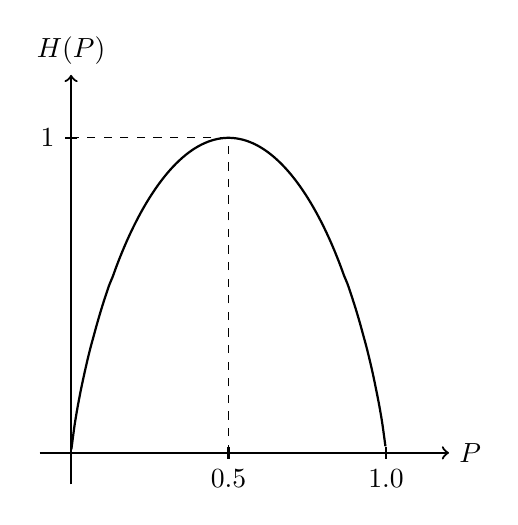
\begin{tikzpicture}[scale=4, thick]
		% Axes
		\draw[->] (-0.1, 0) -- (1.2, 0) node[right] {$P$};
		\draw[->] (0, -0.1) -- (0, 1.2) node[above] {$H(P)$};

		% Ticks
		\draw (0.5, 0.02) -- (0.5, -0.02) node[below] {$0.5$};
		\draw (1, 0.02) -- (1, -0.02) node[below] {$1.0$};
		\draw (0.02, 1) -- (-0.02, 1) node[left] {$1$};

		% Plot H(P)
		\draw[domain=0.001:0.999, samples=100, smooth]
		plot (\x, {-\x * ln(\x)/ln(2) - (1-\x) * ln(1-\x)/ln(2)});

		% Dashed lines for max entropy
		\draw[dashed, thin] (0.5, 0) -- (0.5, 1) -- (0, 1);
	\end{tikzpicture}
	\caption{Entropy $H$ versus Probability $P$}
\end{figure}


Taking antilogarithm on both sides, we get
$$P = 1 - P$$
$$\Rightarrow 2P = 1$$
$$\Rightarrow P = \frac{1}{2}$$

Applying $P = \frac{1}{2}$ in $H = -[P \log P + (1-P) \log (1-P)]$ we get,
$$H_{max} = 1 \text{ bit/message}$$

\subsubsection*{Problems}

\textbf{6.} Consider a source transmitting 6 symbols with probabilities $1/2$, $1/4$, $1/8$, $1/16$, $1/32$, $1/32$. Find the entropy.

\textbf{Ans:}
\begin{align*}
	H & = \sum_{k=1}^{M} P_K \log_2 \left[ \frac{1}{P_K} \right] = \sum_{k=1}^{6} P_K \log_2 \left[ \frac{1}{P_K} \right]                            \\
	  & = \frac{1}{2}\log_2 2 + \frac{1}{4}\log_2 4 + \frac{1}{8}\log_2 8 + \frac{1}{16}\log_2 16 + \frac{1}{32}\log_2 32 + \frac{1}{32}\log_2 32    \\
	  & = \frac{1}{2} \times 1 + \frac{1}{4} \times 2 + \frac{1}{8} \times 3 + \frac{1}{16} \times 4 + \frac{1}{32} \times 5 + \frac{1}{32} \times 5 \\
	  & = \frac{1}{2} + \frac{1}{2} + \frac{3}{8} + \frac{2}{8} + \frac{5}{32} + \frac{5}{32} = \frac{31}{16}                                        \\
	  & = 1.93 \text{ bits/symbol}
\end{align*}

\textbf{7.} Let 'x' represents the outcome of a single roll of a fair die. Find the entropy.

\textbf{Ans:}
$$P_K = \frac{1}{6}$$
$$H = \sum_{k=1}^{M} P_K \log_2 \left[ \frac{1}{P_K} \right] = \sum_{k=1}^{6} P_K \log_2 \left[ \frac{1}{P_K} \right] = 6 \times \frac{1}{6} \log_2[6] = 2.58 \text{ bits/symbol}$$

\vspace{0.5cm}
\noindent \textbf{8.} A source has 5 outputs denoted as $m_1, m_2, m_3, m_4$ \& $m_5$. Their probabilities are 0.3, 0.25, 0.25, 0.15 \& 0.05 respectively. Determine the maximum entropy and the normal entropy of the source.

\textbf{Ans:}
\begin{enumerate}
	\item[i.] For maximum entropy, the messages are of equi-probable. Since there are 5 messages the probability is $P_K = \frac{1}{5}$.
	      $$H = \sum_{k=1}^{M} P_k \log_2 \left[ \frac{1}{P_k} \right] = \sum_{k=1}^{5} P_k \log_2 \left[ \frac{1}{P_k} \right] = 5 \times \frac{1}{5} \log_2[5] = 2.32 \text{ bits/symbol}$$

	\item[ii.] Normal entropy,
	      $$H = \sum_{k=1}^{M} P_K \log_2 \left[ \frac{1}{P_K} \right] = \sum_{k=1}^{5} P_K \log_2 \left[ \frac{1}{P_k} \right]$$
	      \begin{align*}
		       & = 0.3 \log_2 \frac{1}{0.3} + 0.25 \log_2 \frac{1}{0.25} + 0.25 \log_2 \frac{1}{0.25} + 0.15 \log_2 \frac{1}{0.15} + 0.05 \log_2 \frac{1}{0.05} \\
		       & = 0.3 \times 1.737 + 0.25 \times 2 + 0.25 \times 2 + 0.15 \times 2.737 + 0.05 \times 4.32                                                      \\
		       & = 2.14765 \text{ bits/symbol}
	      \end{align*}
\end{enumerate}

\vspace{0.5cm}
\noindent \textbf{9.} A discrete memory-less source produces 5 symbols (R, S, T, U, V) with probabilities $1/3, 1/3, 1/6, 1/9, 1/18$ respectively. Find the average amount of information obtained in the messages RRSTU \& STTUV.

\textbf{Ans:}
\begin{enumerate}
	\item[i.] For RRSTU the entropy is,
	      $$H = \sum_{k=1}^{M} P_k \log_2 \left[ \frac{1}{P_K} \right] = \sum_{k=1}^{5} P_K \log_2 \left[ \frac{1}{P_k} \right]$$
	      \begin{align*}
		      H & = \frac{1}{3}\log_2 3 + \frac{1}{3}\log_2 3 + \frac{1}{3}\log_2 3 + \frac{1}{6}\log_2 6 + \frac{1}{9}\log_2 9 \\
		        & = 0.528 + 0.528 + 0.528 + 0.431 + 0.352 = 2.367 \text{ bits/symbol}
	      \end{align*}

	\item[ii.] For STTUV the entropy is,
	      $$H = \sum_{k=1}^{M} P_k \log_2 \left[ \frac{1}{P_K} \right] = \sum_{k=1}^{5} P_K \log_2 \left[ \frac{1}{P_K} \right]$$
	      \begin{align*}
		      H & = \frac{1}{3}\log_2 3 + \frac{1}{6}\log_2 6 + \frac{1}{6}\log_2 6 + \frac{1}{9}\log_2 9 + \frac{1}{18}\log_2 18 \\
		        & = 0.528 + 0.431 + 0.431 + 0.352 + 0.232 = 1.974 \text{ bits/symbol}
	      \end{align*}
\end{enumerate}

\vspace{0.5cm}
\noindent \textbf{10.} A source produces 8 symbols with equal probability. Find the entropy of the sources. Also determine the entropy if one of the symbols occur with probability $1/2$ while the others occur with equal probability.

\textbf{Ans:}
\begin{enumerate}
	\item[i.] For equal entropy, $P_K = \frac{1}{8}$
	      $$H = \sum_{k=1}^{M} P_k \log_2 \left[ \frac{1}{P_k} \right] = \sum_{k=1}^{8} P_k \log_2 \left[ \frac{1}{P_k} \right] = 8 \times \frac{1}{8} \log_2[8] = 3 \text{ bits/symbols}$$

	\item[ii.] Since the probability of $m_1$ is $\frac{1}{2}$, the other seven messages have the probability $\frac{1}{2}$. Given other 7 messages have equal probability then their probability is $\frac{1}{14}$
	      $$H = \sum_{k=1}^{M} P_k \log_2 \left[ \frac{1}{P_k} \right] = \sum_{k=1}^{8} P_k \log_2 \left[ \frac{1}{P_k} \right]$$
	      $$= \frac{1}{2}\log_2[2] + 7 \times \frac{1}{14}\log_2[14] = 0.5 + 1.9 = 2.4 \text{ bits/symbols}$$
\end{enumerate}

\vspace{0.5cm}
\noindent \textbf{11.} A source produces 2 symbols with equal probability if unbiased. Due to malfunctioning the source produces the combination of symbols as follows: Symbol 1 followed by symbol 2 with a probability of 0.8 \& Symbol 2 followed by symbol 1 with a probability of 0.2. What is the effect on entropy?

\textbf{Ans:} $P(X_1) = \frac{1}{2}$ and $P(X_2) = \frac{1}{2}$ if unbiased.
$$H(X) = 2 \times \frac{1}{2} \log_2 2 = 1 \text{ bit/symbol}$$

Due to malfunctioning
$$P(X_1 X_2) = 0.8 \quad \& \quad P(X_2 X_1) = 0.2$$
\begin{align*}
	H(X) & = \sum_{k=1}^{M} P_k \log_2 \left[ \frac{1}{P_K} \right] = 0.8 \log_2 \left[ \frac{1}{0.8} \right] + 0.2 \log_2 \left[ \frac{1}{0.2} \right] \\
	     & = 0.258 + 0.464 = 0.722 \text{ bits/symbols}
\end{align*}
That is the entropy is reduced to 72.2\%

\subsection{Joint Entropy}
Joint entropy is the average information per pairs of transmitted and received symbols in a communication system. It is denoted as $H(X,Y)$. It is also called system entropy. It is the entropy of a joint event.

Consider two sources $S_1$ \& $S_2$ delivering symbols $x_i$ \& $y_i$ and there may be some dependence between x's and y's. Here we can say the joint entropy of sources $S_1$ \& $S_2$ is $H(X,Y)$.

Now take the case of a communication system. We can say $H(X,Y)$ as the average uncertainty of the whole communication system.

\begin{figure}[ht]
	\centering
	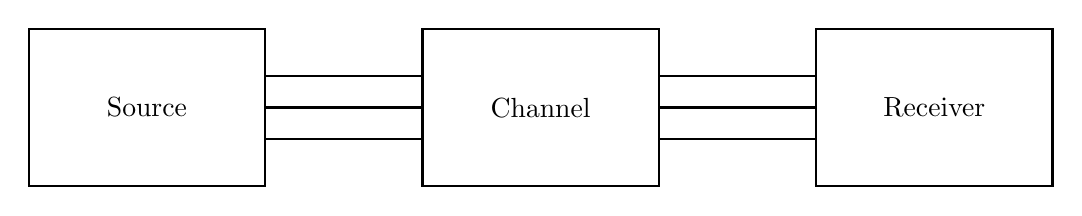
\begin{tikzpicture}[>=stealth, thick]
		% Nodes
		\node[draw, rectangle, minimum width=3cm, minimum height=2cm] (source) at (0,0) {Source};
		\node[draw, rectangle, minimum width=3cm, minimum height=2cm] (channel) at (5,0) {Channel};
		\node[draw, rectangle, minimum width=3cm, minimum height=2cm] (receiver) at (10,0) {Receiver};

		% Connecting lines from Source to Channel
		\draw (source.east) ++(0, 0.4) -- ++(2, 0);
		\draw (source.east) ++(0, 0) -- ++(2, 0);
		\draw (source.east) ++(0, -0.4) -- ++(2, 0);

		% Connecting lines from Channel to Receiver
		\draw (channel.east) ++(0, 0.4) -- ++(2, 0);
		\draw (channel.east) ++(0, 0) -- ++(2, 0);
		\draw (channel.east) ++(0, -0.4) -- ++(2, 0);
	\end{tikzpicture}
	\caption{A Communication System}
\end{figure}

Let the signals transmitted by the source be $x_1, x_2, \ldots, x_i$ and the signals received by the receiver be $y_1, y_2, \ldots, y_j$.
Let there be N symbols in both the transmitter and the receiver.
The probability of the transmitted signals be $P(x_1), P(x_2), \ldots, P(x_i)$ and the probability of the received signals be $P(y_1), P(y_2), \ldots, P(y_j)$.

Then, the entropy of the receiver be
$$H(Y) = \sum_{j=1}^{N} P(y_i) \log_2 \frac{1}{P(y_i)} = - \sum_{j=1}^{N} P(y_i) \log_2 P(y_i)$$

Similarly, the joint entropy be
$$H(X,Y) = - \sum_{i=1}^{N} \sum_{j=1}^{N} P(x_i, y_i) \log_2 P(x_i, y_i) \quad \ldots\ldots(1)$$

According to the probability theory, if A \& B are dependent events, then
$$P(AB) = P(A)P(B|A) \quad \ldots\ldots(2)$$
or
$$P(AB) = P(B)P(A|B) \quad \ldots\ldots(3)$$

Applying (2) in (1), we get
\begin{align*}
	H(X,Y) & = - \sum_{i=1}^{N} \sum_{j=1}^{N} P(x_i) P(y_i|x_i) \log_2 [P(x_i) P(y_i|x_i)]                                                        \\
	       & = - \sum_{i=1}^{N} \sum_{j=1}^{N} P(x_i) P(y_i|x_i) \log_2 P(x_i) - \sum_{i=1}^{N} \sum_{j=1}^{N} P(x_i) P(y_i|x_i) \log_2 P(y_i|x_i) \\
	       & = - \sum_{i=1}^{N} \sum_{j=1}^{N} P(x_i, y_i) \log_2 P(x_i) - \sum_{i=1}^{N} \sum_{j=1}^{N} P(x_i, y_i) \log_2 P(y_i|x_i)             \\
	       & = H(X) + H(Y|X)
\end{align*}

Similarly, by applying (3) in (1), we get
$$H(X,Y) = H(Y) + H(X|Y)$$

$$H(X,Y) = H(X) + H(Y|X)$$
$$H(X,Y) = H(Y) + H(X|Y)$$

\textbf{Note:}
On expanding $-\sum_{i=1}^N \sum_{j=1}^N P\left(x_i\right) P\left(y_i | x_i\right) \log _2 P\left(x_i\right)$, we get
$$
	\begin{aligned}
		 & = -\sum_{i=1}^N\left[\sum_{j=1}^N P\left(x_i\right) P\left(y_i | x_i\right) \log _2 P\left(x_i\right)\right]                                                                       \\
		 & =-\sum_{i=1}^N\left[
			P\left(x_i\right) P\left(y_1 | x_i\right) \log _2 P\left(x_i\right)+
			P\left(x_i\right) P\left(y_2 | x_i\right) \log _2 P\left(x_i\right)+
			\ldots +
		P\left(x_i\right) P\left(y_N | x_i\right) \log _2 P\left(x_i\right)\right]                                                                                                            \\
		 & =-\left[\begin{array}{l}
				           P\left(x_1\right) P\left(y_1 | x_1\right) \log _2 P\left(x_1\right)+
				           P\left(x_2\right) P\left(y_1 | x_2\right) \log _2 P\left(x_2\right)+
				           \ldots +
				           \\
				           P\left(x_1\right) P\left(y_2 | x_1\right) \log _2 P\left(x_1\right)+
				           P\left(x_2\right) P\left(y_2 | x_2\right) \log _2 P\left(x_2\right)+
				           \ldots + \\
				           \vdots   \\
				           P\left(x_1\right) P\left(y_N | x_1\right) \log _2 P\left(x_1\right)+
				           P\left(x_2\right) P\left(y_N | x_2\right) \log _2 P\left(x_2\right)+ \ldots
			           \end{array}\right]                                                                                                 \\
		 & =-\left[\begin{array}{l}
				           P\left(x_1\right) \log_2 P\left(x_1\right) \left[\begin{array}{l}P\left(y_1 | x_1\right) + P\left(y_2 | x_1\right) + \ldots + P\left(y_N | x_1\right) \end{array}\right] + \\
				           P\left(x_2\right) \log_2 P\left(x_2\right) \left[\begin{array}{l}P\left(y_1 | x_2\right) + P\left(y_2 | x_2\right) + \ldots + P\left(y_N | x_2\right) \end{array}\right] + \\
				           \vdots                                                                                                                                                                     \\
				           P\left(x_N\right) \log_2 P\left(x_N\right) \left[\begin{array}{l}P\left(y_1 | x_N\right) + P\left(y_2 | x_N\right) + \ldots + P\left(y_N | x_N\right) \end{array}\right] + \\
			           \end{array}\right] \\
		 & =-\left[P\left(x_1\right) \log _2 P\left(x_1\right)+P\left(x_2\right) \log _2 P\left(x_2\right)+\ldots \ldots+P\left(x_N\right) \log _2 P\left(x_N\right)\right]                   \\
		 & =-\sum_{i=1}^N P\left(x_i\right) \log _2 P\left(x_i\right)=H(X)
	\end{aligned}
$$

Similarly, we can prove $-\sum_{i=1}^N \sum_{j=1}^N P\left(x_i, y_i\right) \log _2 P\left(y_i / x_i\right)=H(Y / X)$

\subsection{Conditional Entropy}

Conditional entropy means the entropy of a subsystem when the state of another subsystem is known, where the two systems are statically correlated. In a communication system, we usually denote the conditional entropy as $H(X|Y)$ or $H(Y|X)$.

$H(Y|X)$ is the entropy of the received symbols when the transmitter state is known. That is, it is the amount of uncertainty remaining in the channel output after the channel output has been sent.

$H(X|Y)$ is the entropy of the source when the received state is known.

The conditional entropy of '$X$' when given $Y=y_j$ can be found out by the basic equation of entropy:
$$H = \sum_{k=1}^{M} P_k \log_2 \frac{1}{P_k}$$

Thus for $H(X|Y=y_j)$,
$$H(X|Y=y_j) = \sum_{i=1}^{M} P(x_i|y_j) \log_2 \frac{1}{P(x_i|y_j)}$$

This quantity is a random variable that takes on values $H(X|Y=y_1)$, $H(X|Y=y_2) \dots$ with probabilities $P(y_1)$, $P(y_2) \dots$ respectively.

Thus the mean entropy is given by,
\begin{align*}
	H(X|Y) & = \sum_{j=1}^{N} H(X|Y=y_j) P(y_j)                                                           \\
	       & = \sum_{i=1}^{M} \sum_{j=1}^{N} P(x_i|y_j) \log_2 \left[ \frac{1}{P(x_i|y_j)} \right] P(y_j) \\
	       & = \sum_{i=1}^{M} \sum_{j=1}^{N} P(x_i|y_j) P(y_j) \log_2 \left[ \frac{1}{P(x_i|y_j)} \right] \\
	       & = \sum_{i=1}^{M} \sum_{j=1}^{N} P(x_i, y_j) \log_2 \left[ \frac{1}{P(x_i|y_j)} \right]
\end{align*}

Similarly we get,
$$H(Y|X) = - \sum_{i=1}^{M} \sum_{j=1}^{N} P(x_i, y_j) \log_2 P(y_j|x_i)$$

\subsection{Marginal Entropy}
Marginal entropy is the entropy of the source. It is denoted by $H(X)$.

\subsection{Receiver Entropy}
Receiver entropy is the entropy of the receiver. It is denoted by $H(Y)$.

\textbf{Note:}
\begin{enumerate}
	\item[i.] \textbf{Equivocation}\\
	      Equivocation means loss of information due to channel.
	\item[ii.] \textbf{Transition Matrix (Noise Matrix or Channel Matrix)}\\
	      It is the matrix of $P(Y|X)$
	      $$P(Y|X) = \begin{bmatrix}
			      P(y_1|x_1) & P(y_2|x_1) \\
			      P(y_1|x_2) & P(y_2|x_2)
		      \end{bmatrix}$$
\end{enumerate}

\subsubsection*{Problems}

\textbf{12.} Consider a source with alphabets $X_1, X_2, X_3$ \& $X_4$ with probabilities $P(X) = \{1/2, 1/4, 1/8, 1/8\}$. Find the entropy for second order extension?

\textbf{Ans:}
\begin{align*}
	H(X) & = \sum P(X) \log_2 \left[ \frac{1}{P(X)} \right]                                            \\
	     & = \frac{1}{2}\log_2[2] + \frac{1}{4}\log_2[4] + \frac{1}{8}\log_2[8] + \frac{1}{8}\log_2[8] \\
	     & = \frac{1}{2} + \frac{1}{2} + \frac{3}{8} + \frac{3}{8} = 1.75 \text{ bits/symbol}
\end{align*}

\textbf{For Second Order Extension}

\begin{table}[ht]
	\centering
	\renewcommand{\arraystretch}{1.5}
	\begin{tabular}{|l|c|c|c|c|c|c|c|c|}
		\hline
		\cellcolor{black!10}\textbf{Symbols of $S^2$} & $Y_1$         & $Y_2$         & $Y_3$          & $Y_4$          & $Y_5$         & $Y_6$          & $Y_7$          & $Y_8$          \\ \hline
		\cellcolor{black!10}\textbf{Alphabets}        & $X_1X_1$      & $X_1X_2$      & $X_1X_3$       & $X_1X_4$       & $X_2X_1$      & $X_2X_2$       & $X_2X_3$       & $X_2X_4$       \\ \hline
		\cellcolor{black!10}\textbf{Probability}      & $\frac{1}{4}$ & $\frac{1}{8}$ & $\frac{1}{16}$ & $\frac{1}{16}$ & $\frac{1}{8}$ & $\frac{1}{16}$ & $\frac{1}{32}$ & $\frac{1}{32}$ \\ \hline
	\end{tabular}%
	\vspace{0.2cm}

	\begin{tabular}{|l|c|c|c|c|c|c|c|c|}
		\hline
		\cellcolor{black!10}\textbf{Symbols of $S^2$} & $Y_9$          & $Y_{10}$       & $Y_{11}$       & $Y_{12}$       & $Y_{13}$       & $Y_{14}$       & $Y_{15}$       & $Y_{16}$       \\ \hline
		\cellcolor{black!10}\textbf{Alphabets}        & $X_3X_1$       & $X_3X_2$       & $X_3X_3$       & $X_3X_4$       & $X_4X_1$       & $X_4X_2$       & $X_4X_3$       & $X_4X_4$       \\ \hline
		\cellcolor{black!10}\textbf{Probability}      & $\frac{1}{16}$ & $\frac{1}{32}$ & $\frac{1}{64}$ & $\frac{1}{64}$ & $\frac{1}{16}$ & $\frac{1}{32}$ & $\frac{1}{64}$ & $\frac{1}{64}$ \\ \hline
	\end{tabular}%
\end{table}

\begin{align*}
	H(X^2) & = \sum P(Y) \log_2 \left[ \frac{1}{P(Y)} \right]                                                                                                                             \\
	       & = \frac{1}{4}\log_2[4] + \frac{1}{8}\log_2[8] + \frac{1}{16}\log_2[16] + \frac{1}{16}\log_2[16] + \frac{1}{8}\log_2[8] + \frac{1}{16}\log_2[16]                              \\
	       & \quad + \frac{1}{32}\log_2[32] + \frac{1}{32}\log_2[32] + \frac{1}{16}\log_2[16] + \frac{1}{32}\log_2[32] + \frac{1}{64}\log_2[64]                                           \\
	       & \quad + \frac{1}{64}\log_2[64] + \frac{1}{16}\log_2[16] + \frac{1}{32}\log_2[32] + \frac{1}{64}\log_2[64] + \frac{1}{64}\log_2[64]                                           \\
	       & = \frac{1}{2} + \frac{3}{8} + \frac{1}{4} + \frac{1}{4} + \frac{3}{8} + \frac{1}{4} + \frac{5}{32} + \frac{5}{32} + \frac{1}{4} + \frac{5}{32} + \frac{3}{32} + \frac{3}{32} \\
	       & \quad + \frac{1}{4} + \frac{5}{32} + \frac{3}{32} + \frac{3}{32} = 3.5 \text{ bits/symbol}
\end{align*}

From this, $H(X^2) = 2 H(X)$.

\vspace{0.5cm}
\textbf{13.} Consider a source with messages 0 \& 1 with probabilities $P(0) = 0.25$ \& $P(1) = 0.75$. Find the third order extension of the source?

\textbf{Ans:}
\begin{align*}
	H(X) & = \sum P(X) \log_2 \left[ \frac{1}{P(X)} \right]                                                                                        \\
	     & = \frac{1}{4}\log_2[4] + \frac{3}{4}\log_2\left[\frac{4}{3}\right] = \frac{1}{2} + \frac{3}{4} \times 0.415 = 0.811 \text{ bits/symbol}
\end{align*}

\begin{table}[ht]
	\centering
	\renewcommand{\arraystretch}{1.5}
	\begin{tabular}{|l|c|c|c|c|c|c|c|c|}
		\hline
		\cellcolor{black!10}\textbf{Symbols of $S^3$} & $Y_1$          & $Y_2$          & $Y_3$          & $Y_4$          & $Y_5$          & $Y_6$          & $Y_7$          & $Y_8$           \\ \hline
		\cellcolor{black!10}\textbf{Alphabets}        & $000$          & $001$          & $010$          & $011$          & $100$          & $101$          & $110$          & $111$           \\ \hline
		\cellcolor{black!10}\textbf{Probability}      & $\frac{1}{64}$ & $\frac{3}{64}$ & $\frac{3}{64}$ & $\frac{9}{64}$ & $\frac{3}{64}$ & $\frac{9}{64}$ & $\frac{9}{64}$ & $\frac{27}{64}$ \\ \hline
	\end{tabular}
\end{table}

\begin{align*}
	H(X^3) & = \sum P(Y) \log_2 \left[ \frac{1}{P(Y)} \right]                                                                                                                                                \\
	       & = \frac{1}{64}\log_2[64] + \frac{3}{64}\log_2\left[\frac{64}{3}\right] + \frac{3}{64}\log_2\left[\frac{64}{3}\right] + \frac{9}{64}\log_2\left[\frac{64}{9}\right]                              \\
	       & \quad + \frac{3}{64}\log_2\left[\frac{64}{3}\right] + \frac{9}{64}\log_2\left[\frac{64}{9}\right] + \frac{9}{64}\log_2\left[\frac{64}{9}\right] + \frac{27}{64}\log_2\left[\frac{64}{27}\right] \\
	       & = 0.094 + 0.207 + 0.207 + 0.378 + 0.207 + 0.378 + 0.378 + 0.525                                                                                                                                 \\
	       & = 2.445 \text{ bits/symbol}
\end{align*}

From this $H(X^3) = 3 H(X)$.
So in General, $H(X^n) = n H(X)$.

\vspace{0.5cm}
\textbf{14.} Consider that two sources emit messages $x_1, x_2, x_3$ and $y_1, y_2, y_3$ with joint probability $P(X,Y)$ as shown in the matrix form. Calculate $H(X)$, $H(Y)$, $H(X|Y)$ and $H(Y|X)$?

\textbf{Ans:}

\begin{flalign*}
	\setlength{\arraycolsep}{5pt}
	\renewcommand\arraystretch{2}
	P(X,Y) =
	\begin{bmatrix}
		3/40 & 1/40 & 1/40 \\
		1/20 & 3/20 & 1/20 \\
		1/8  & 1/8  & 3/8
	\end{bmatrix}
\end{flalign*}

\begin{enumerate}
	\item[i.] \textbf{To find $H(X)$}
	      \begin{flalign*}
		      P(X_1) & = \frac{3}{40} + \frac{1}{40} + \frac{1}{40} = \frac{5}{40} = \frac{1}{8} &  & \\
		      P(X_2) & = \frac{1}{20} + \frac{3}{20} + \frac{1}{20} = \frac{5}{20} = \frac{1}{4} &  & \\
		      P(X_3) & = \frac{1}{8} + \frac{1}{8} + \frac{3}{8} = \frac{5}{8}                   &  &
	      \end{flalign*}
	      \begin{flalign*}
		      H(X) & = \sum P(X) \log_2 \left[ \frac{1}{P(X)} \right] = \frac{1}{8}\log_2[8] + \frac{1}{4}\log_2[4] + \frac{5}{8}\log_2\left[\frac{8}{5}\right] &  & \\
		           & = \frac{1}{8}\times 3 + \frac{1}{4}\times 2 + \frac{5}{8}\times 0.6781                                                                     &  & \\
		           & = 1.3 \text{ bits/symbols}                                                                                                                 &  &
	      \end{flalign*}

	\item[ii.] \textbf{To find $H(Y)$}
	      \begin{flalign*}
		      P(Y_1) & = \frac{3}{40} + \frac{1}{20} + \frac{1}{8} = 0.25 &  & \\
		      P(Y_2) & = \frac{1}{40} + \frac{3}{20} + \frac{1}{8} = 0.3  &  & \\
		      P(Y_3) & = \frac{1}{40} + \frac{1}{20} + \frac{3}{8} = 0.45 &  &
	      \end{flalign*}
	      \begin{flalign*}
		      H(Y) & = \sum P(Y) \log_2 \left[ \frac{1}{P(Y)} \right]                                                                         &  & \\
		           & = 0.25 \log_2\left[\frac{1}{0.25}\right] + 0.3 \log_2\left[\frac{1}{0.3}\right] + 0.45 \log_2\left[\frac{1}{0.45}\right] &  & \\
		           & = 0.5 + 0.52 + 0.52                                                                                                      &  & \\
		           & = 1.54 \text{ bits/symbols}                                                                                              &  &
	      \end{flalign*}

	\item[iii.] \textbf{To find $H(X|Y)$}
	      We have $P(X|Y) = \dfrac{P(X,Y)}{P(Y)}$
	      \begin{align*}
		      H(X|Y) & = \sum_i \sum_j P(X,Y) \log_2 \left[ \frac{1}{P(X|Y)} \right]                                                                                                         &  & \\
		             & = \frac{3}{40}\log_2\left[\frac{10}{3}\right] + \frac{1}{40}\log_2[12] + \frac{1}{40}\log_2[18] + \frac{1}{20}\log_2[5]                                               &  & \\
		             & \quad + \frac{3}{20}\log_2[2] + \frac{1}{20}\log_2[9] + \frac{1}{8}\log_2[2] + \frac{1}{8}\log_2\left[\frac{12}{5}\right] + \frac{3}{8}\log_2\left[\frac{6}{5}\right] &  & \\
		             & = 0.13 + 0.09 + 0.10 + 0.12 + 0.15 + 0.16 + 0.13 + 0.16 + 0.10                                                                                                        &  & \\
		             & = 1.14 \text{ bits/symbols}                                                                                                                                           &  &
	      \end{align*}

	\item[iv.] \textbf{To find $H(Y|X)$}
	      We have $P(Y|X) = \dfrac{P(X,Y)}{P(X)}$
\end{enumerate}

\begin{align*}
	H(Y|X) & = \sum_i \sum_j P(X,Y) \log_2 \left[ \frac{1}{P(Y|X)} \right]                                                                                                        &  & \\
	       & = \frac{3}{40}\log_2\left[\frac{5}{3}\right] + \frac{1}{40}\log_2[5] + \frac{1}{40}\log_2[5] + \frac{1}{20}\log_2[5]                                                 &  & \\
	       & \quad + \frac{3}{20}\log_2\left[\frac{5}{3}\right] + \frac{1}{20}\log_2[5] + \frac{1}{8}\log_2[5] + \frac{1}{8}\log_2[5] + \frac{3}{8}\log_2\left[\frac{5}{3}\right] &  & \\
	       & = 0.06 + 0.06 + 0.06 + 0.12 + 0.11 + 0.12 + 0.29 + 0.29 + 0.28                                                                                                       &  & \\
	       & = 1.39 \text{ bits/symbols}                                                                                                                                          &  &
\end{align*}


\vspace{0.5cm}
\noindent \textbf{15.} Consider a channel with two inputs $X_1, X_2$ and three outputs $Y_1, Y_2, Y_3$ and the transition matrix of the channel is given by
$$P(Y|X) = \begin{blockarray}{cccc}
		& Y_1 & Y_2 & Y_3 \\
		\begin{block}{c[ccc]}
			X_1 & 3/4 & 1/4 & 0 \\
			X_2 & 0 & 1/2 & 1/2 \\
		\end{block}
	\end{blockarray}$$

Calculate $H(X), H(Y), H(X|Y)$ and $H(Y|X)$. Given $P(X_1) = 1/2$, $P(X_2) = 1/2$.

\textbf{Ans:}

We have $P(X,Y) = P(X)P(Y|X)$
\begin{align*}
	P(X_1, Y_1) & = P(X_1)P(Y_1|X_1) = \frac{1}{2} \times \frac{3}{4} = \frac{3}{8}      \\
	P(X_1, Y_2) & = P(X_1)P(Y_2|X_1) = \frac{1}{2} \times \frac{1}{4} = \frac{1}{8}      \\
	P(X_1, Y_3) & = 0                                                                    \\
	P(X_2, Y_1) & = 0                                                                    \\
	P(X_2, Y_2) & = P(X_2)P(Y_2|X_2) = \frac{1}{2} \times \frac{1}{2} = \frac{1}{4}      \\
	P(X_2, Y_3) & = P(X_2)P(Y_3|X_2) = \frac{1}{2} \times \frac{1}{2} = \frac{1}{4} &  &
\end{align*}

$$P(X,Y) = \begin{blockarray}{cccc}
		& Y_1 & Y_2 & Y_3 \\
		\begin{block}{c[ccc]}
			X_1 & 3/8 & 1/8 & 0 \\
			X_2 & 0 & 1/4 & 1/4 \\
		\end{block}
	\end{blockarray}$$

\begin{enumerate}
	\item[i.] \textbf{To find $H(X)$}
	      \begin{align*}
		      P(X_1) & = \frac{3}{8} + \frac{1}{8} = \frac{4}{8} = \frac{1}{2} \\
		      P(X_2) & = \frac{1}{4} + \frac{1}{4} = \frac{1}{2}
	      \end{align*}
	      $$H(X) = \sum P(X) \log_2 \left[ \frac{1}{P(X)} \right] = \frac{1}{2}\log_2[2] + \frac{1}{2}\log_2[2] = \frac{1}{2} + \frac{1}{2} = 1 \text{ bits/symbol}$$

	\item[ii.] \textbf{To find $H(Y)$}
	      \begin{align*}
		      P(Y_1) & = \frac{3}{8}; \quad P(Y_2) = \frac{1}{4} + \frac{1}{8} = \frac{3}{8}; \quad P(Y_3) = \frac{1}{4}
	      \end{align*}
	      \begin{align*}
		      H(Y) & = \sum P(Y) \log_2 \left[ \frac{1}{P(Y)} \right] = \frac{3}{8}\log_2\left[\frac{8}{3}\right] + \frac{3}{8}\log_2\left[\frac{8}{3}\right] + \frac{1}{4}\log_2[4] \\
		           & = 0.52 + 0.52 + 0.5 = 1.54 \text{ bits/symbols}
	      \end{align*}

	\item[iii.] \textbf{To find $H(X|Y)$}
	      We have $P(X|Y) = \dfrac{P(X,Y)}{P(Y)} = \begin{bmatrix} 1 & 1/3 & 0 \\ 0 & 2/3 & 1 \end{bmatrix}$
	      \begin{align*}
		      H(X|Y) & = \sum_i \sum_j P(X,Y) \log_2 \left[ \frac{1}{P(X|Y)} \right]                                                    \\
		             & = \frac{3}{8}\log_2[1] + \frac{1}{8}\log_2[3] + \frac{1}{4}\log_2\left[\frac{3}{2}\right] + \frac{1}{4}\log_2[1] \\
		             & = \frac{1}{8} \times 1.585 + \frac{1}{4} \times 0.58 = 0.343 \text{ bits/symbols}
	      \end{align*}

	\item[iv.] \textbf{To find $H(Y|X)$}
	      \begin{align*}
		      H(Y|X) & = \sum_i \sum_j P(X,Y) \log_2 \left[ \frac{1}{P(Y|X)} \right]                                                    \\
		             & = \frac{3}{8}\log_2\left[\frac{4}{3}\right] + \frac{1}{8}\log_2[4] + \frac{1}{4}\log_2[2] + \frac{1}{4}\log_2[2] \\
		             & = 0.155 + 0.25 + 0.25 + 0.25 = 0.905 \text{ bits/symbols}
	      \end{align*}
\end{enumerate}


\vspace{0.5cm}
\noindent \textbf{16.} Show that the marginal entropy is greater than or equal to the conditional entropy, i.e. $H(X) \ge H(X|Y)$.

\textbf{Ans:} For this proof, consider the plots given below:

\begin{figure}[ht]
	\centering
	\begin{tikzpicture}[scale=2.5, thick]
		% Axes
		\draw[->] (-0.2, 0) -- (2.5, 0) node[right] {$x$};
		\draw[->] (0, -1.2) -- (0, 1.2);

		% Ticks
		\draw (1, 0.05) -- (1, -0.05) node[below] {$1.0$};
		\draw (2, 0.05) -- (2, -0.05) node[below] {$2.0$};
		\draw (0.05, 1) -- (-0.05, 1) node[left] {$1.0$};
		\draw (0.05, -1) -- (-0.05, -1) node[left] {$-1.0$};

		% Plot y = x - 1
		\draw (0, -1) -- (2.1, 1.1) node[above left, xshift=-0.5cm] {$y = x - 1$};

		% Plot y = ln(x)
		\draw[domain=0.25:2.3, samples=100] plot (\x, {ln(\x)}) node[below right, xshift=-0.3cm] {$y = \log x$};
	\end{tikzpicture}
	\caption{Graphs of the functions $x - 1$ and $\log x$ versus $x$}
\end{figure}

The figure shows the plots of a straight line $y = x - 1$ and a logarithmic function $y = \ln x$ on the same set of co-ordinate axis. Note that, any point on the straight line will always be above the logarithmic function for any given value of $x$.

$$ \therefore \ln x \le x - 1 $$

Multiplying both sides by -1, we get,
\begin{align*}
	-\ln x                      & \ge -(x - 1) \\
	\Rightarrow \ln x^{-1}      & \ge 1 - x    \\
	\Rightarrow \ln \frac{1}{x} & \ge 1 - x
\end{align*}

Take $H(X) - H(X|Y)$:
\begin{align*}
	H(X) - H(X|Y) & = - \sum_i P(x_i) \ln P(x_i) + \sum_i \sum_j P(x_i, y_j) \ln P(x_i|y_j)             \\
	              & = - \sum_i \sum_j P(x_i, y_j) \ln P(x_i) + \sum_i \sum_j P(x_i, y_j) \ln P(x_i|y_j) \\
	              & = \sum_i \sum_j P(x_i, y_j) \left[ \ln P(x_i|y_j) - \ln P(x_i) \right]              \\
	              & = \sum_i \sum_j P(x_i, y_j) \left[ \ln \frac{P(x_i|y_j)}{P(x_i)} \right]
\end{align*}

We have $\left[ \ln \dfrac{P(x_i|y_j)}{P(x_i)} \right] \ge 1 - \dfrac{P(x_i)}{P(x_i|y_j)}$

So,
\begin{align*}
	H(X) - H(X|Y) & \ge \sum_i \sum_j P(x_i, y_j) \left[ 1 - \frac{P(x_i)}{P(x_i|y_j)} \right]                     \\
	              & \ge \sum_i \sum_j \left[ P(x_i, y_j) - P(x_i, y_j) \frac{P(x_i)}{P(x_i|y_j)} \right]           \\
	              & \ge \sum_i \sum_j \left[ P(x_i, y_j) - P(x_i, y_j) \frac{P(x_i)}{P(x_i, y_j) / P(y_j)} \right] \\
	              & \ge \sum_i \sum_j \left[ P(x_i, y_j) - P(x_i)P(y_j) \right]                                    \\
	              & \ge \sum_i \sum_j P(x_i, y_j) - \sum_i \sum_j P(x_i)P(y_j)                                     \\
	              & \ge 1 - 1                                                                                      \\
	H(X) - H(X|Y) & \ge 0
\end{align*}

So, $H(X) \ge H(X|Y)$

\subsection{Mutual Information}
It is the information obtained when we have a prior knowledge or a posterior knowledge regarding the information or the loss of information. Consider the initial uncertainty about the source is $H(X)$ and the final uncertainty about reception is $H(X|Y)$. Then $I(X,Y)$ is the mutual information given by:
$$I(X,Y) = H(X) - H(X|Y) \text{ bits/symbol}$$

\begin{align*}
	I(X,Y) & = \sum_{i=1}^{N} \sum_{j=1}^{N} P(x_i, y_i) \log_2 \left( \frac{1}{P(x_i)} \right) - \sum_{i=1}^{N} \sum_{j=1}^{N} P(x_i, y_i) \log_2 \left[ \frac{1}{P(x_i|y_i)} \right] \\
	       & = \sum_{i=1}^{N} \sum_{j=1}^{N} P(x_i, y_i) \left[ \log_2 \left( \frac{1}{P(x_i)} \right) - \log_2 \left( \frac{1}{P(x_i|y_i)} \right) \right]                            \\
	       & = \sum_{i=1}^{N} \sum_{j=1}^{N} P(x_i, y_i) \left[ -\log_2 (P(x_i)) + \log_2 (P(x_i|y_i)) \right]                                                                         \\
	       & = \sum_{i=1}^{N} \sum_{j=1}^{N} P(x_i, y_i) \left[ \log_2 \left( \frac{P(x_i|y_i)}{P(x_i)} \right) \right]
\end{align*}

If we substitute $P(X|Y) = \dfrac{P(X,Y)}{P(Y)}$,
$$I(X,Y) = \sum_{i=1}^{N} \sum_{j=1}^{N} P(x_i, y_i) \left[ \log_2 \left( \frac{P(x_i, y_i)}{P(x_i) \times P(y_i)} \right) \right]$$

If we substitute $\dfrac{P(X,Y)}{P(X)} = P(Y|X)$,
\begin{align*}
	I(X,Y) & = \sum_{i=1}^{N} \sum_{j=1}^{N} P(x_i, y_i) \left[ \log_2 \left( \frac{P(y_i|x_i)}{P(y_i)} \right) \right]                                                                \\
	       & = \sum_{i=1}^{N} \sum_{j=1}^{N} P(x_i, y_i) \log_2 \left( \frac{1}{P(y_i)} \right) - \sum_{i=1}^{N} \sum_{j=1}^{N} P(x_i, y_i) \log_2 \left( \frac{1}{P(y_i|x_i)} \right) \\
	       & = H(Y) - H(Y|X)
\end{align*}

$$I(X,Y) = H(X) - H(X|Y) = H(Y) - H(Y|X)$$

\begin{figure}[ht]
	\centering
	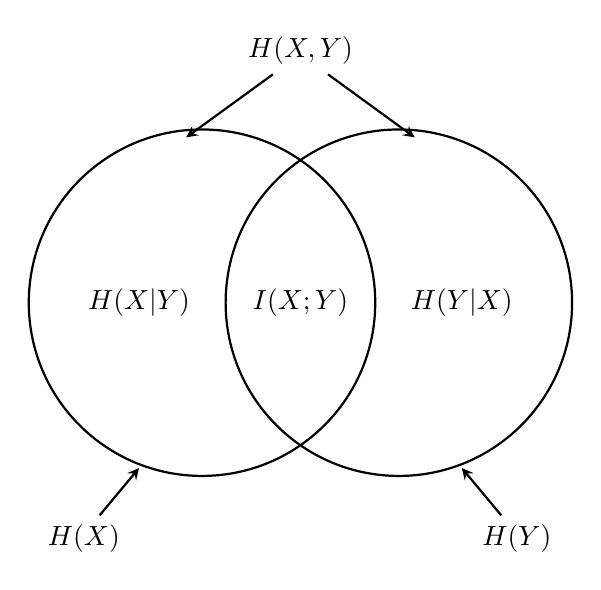
\begin{tikzpicture}[thick]
		% Circles
		\draw (0,0) circle (2.2cm);
		\draw (2.5,0) circle (2.2cm);

		% Text inside circles
		\node at (-0.8,0) {$H(X|Y)$};
		\node at (1.25,0) {$I(X;Y)$};
		\node at (3.3,0) {$H(Y|X)$};

		% H(X,Y) Label
		\node at (1.25, 3.2) {$H(X,Y)$};
		\draw[->, >=stealth] (0.9, 2.9) -- (-0.2, 2.1);
		\draw[->, >=stealth] (1.6, 2.9) -- (2.7, 2.1);

		% H(X) and H(Y) Labels
		\node at (-1.5, -3) {$H(X)$};
		\draw[->, >=stealth] (-1.3, -2.7) -- (-0.8, -2.1);

		\node at (4, -3) {$H(Y)$};
		\draw[->, >=stealth] (3.8, -2.7) -- (3.3, -2.1);
	\end{tikzpicture}
	\caption{Relationship between entropy and mutual information.}
\end{figure}

\vspace{0.5cm}
\noindent \textbf{17.} Given the joint probability matrix:
$$P(X,Y) = \begin{blockarray}{ccccc}
		& Y_1 & Y_2 & Y_3 & Y_4 \\
		\begin{block}{c[cccc]}
			X_1 & 1/4 & 0 & 0 & 0 \\
			X_2 & 1/10 & 3/10 & 0 & 0 \\
			X_3 & 0 & 1/20 & 1/10 & 0 \\
			X_4 & 0 & 0 & 1/20 & 1/10 \\
			X_5 & 0 & 0 & 1/20 & 0 \\
		\end{block}
	\end{blockarray}$$

With probabilities of source alphabet $P(X) = \{1/4, 2/5, 3/20, 3/20, 1/20\}$. Find the values of $H(X)$, $H(Y)$, $H(X|Y)$, $H(Y|X)$ and $I(X,Y)$.

\textbf{Ans:}
\begin{enumerate}
	\item[i.] \textbf{To find $H(X)$}
	      \begin{align*}
		      P(X_1) & = \frac{1}{4}; \quad P(X_2) = \frac{1}{10} + \frac{3}{10} = \frac{4}{10} = \frac{2}{5};                  \\
		      P(X_3) & = \frac{1}{20} + \frac{1}{10} = \frac{3}{20}; \quad P(X_4) = \frac{1}{20} + \frac{1}{10} = \frac{3}{20}; \\
		      P(X_5) & = \frac{1}{20}
	      \end{align*}
	      \begin{align*}
		      H(X) & = \sum P(X) \log_2 \left[ \frac{1}{P(X)} \right]                                                                                                                                        \\
		           & = \frac{1}{4}\log_2[4] + \frac{2}{5}\log_2\left[\frac{5}{2}\right] + \frac{3}{20}\log_2\left[\frac{20}{3}\right] + \frac{3}{20}\log_2\left[\frac{20}{3}\right] + \frac{1}{20}\log_2[20] \\
		           & = \frac{2}{4} + 0.528 + 0.410 + 0.410 + 0.216 = 2.06 \text{ bits/symbols}
	      \end{align*}

	\item[ii.] \textbf{To find $H(Y)$}
	      \begin{align*}
		      P(Y_1) & = \frac{1}{4} + \frac{1}{10} = \frac{7}{20}; \quad P(Y_2) = \frac{3}{10} + \frac{1}{20} = \frac{7}{20}; \\
		      P(Y_3) & = \frac{1}{10} + \frac{1}{20} + \frac{1}{20} = \frac{1}{5}; \quad P(Y_4) = \frac{1}{10}
	      \end{align*}
	      \begin{align*}
		      H(Y) & = \sum P(Y) \log_2 \left[ \frac{1}{P(Y)} \right]                                                                                            \\
		           & = \frac{7}{20}\log_2\left[\frac{20}{7}\right] + \frac{7}{20}\log_2\left[\frac{20}{7}\right] + \frac{1}{5}\log_2[5] + \frac{1}{10}\log_2[10] \\
		           & = 0.53 + 0.53 + 0.46 + 0.33 = 1.856 \text{ bits/symbols}
	      \end{align*}

	\item[iii.] \textbf{To find $H(X|Y)$}
	      We have $P(X|Y) = \dfrac{P(X,Y)}{P(Y)}$
	      \begin{align*}
		      H(X|Y) & = \sum_i \sum_j P(X,Y) \log_2 \left[ \frac{1}{P(X|Y)} \right]                                                                                                                         \\
		             & = \frac{1}{4}\log_2\left[\frac{7}{5}\right] + \frac{1}{10}\log_2\left[\frac{7}{2}\right] + \frac{3}{10}\log_2\left[\frac{7}{6}\right] + \frac{1}{20}\log_2[7] + \frac{1}{10}\log_2[2] \\
		             & \quad + \frac{1}{20}\log_2[4] + \frac{1}{10}\log_2[1] + \frac{1}{20}\log_2[4]                                                                                                         \\
		             & = 0.121 + 0.180 + 0.066 + 0.140 + 0.1 + 0.1 + 0.1 = 0.807 \text{ bits/symbols}
	      \end{align*}

	\item[iv.] \textbf{To find $H(Y|X)$}
	      We have $P(Y|X) = \dfrac{P(X,Y)}{P(X)}$
	      \begin{align*}
		      H(Y|X) & = \sum_i \sum_j P(X,Y) \log_2 \left[ \frac{1}{P(Y|X)} \right]                                                                                                                                              \\
		             & = \frac{1}{4}\log_2[1] + \frac{1}{10}\log_2\left[\frac{1}{4}\right] + \frac{3}{10}\log_2\left[\frac{3}{4}\right] + \frac{1}{20}\log_2\left[\frac{1}{3}\right] + \frac{1}{10}\log_2\left[\frac{2}{3}\right] \\
		             & \quad + \frac{1}{20}\log_2\left[\frac{1}{3}\right] + \frac{1}{10}\log_2\left[\frac{2}{3}\right] + \frac{1}{20}\log_2[1]                                                                                    \\
		             & = 0 + 0.2 + 0.1245 + 0.079 + 0.058 + 0.079 + 0 = 0.5995 \text{ bits/symbols}
	      \end{align*}

	\item[v.] \textbf{To find $I(X,Y)$}
	      \begin{align*}
		      I(X,Y) & = H(X) - H(X|Y) = H(Y) - H(Y|X)             \\
		             & = 2.06 - 0.807 = 1.253 \text{ bits/symbols}
	      \end{align*}
\end{enumerate}

\section{Rate of Information}
The rate of information is defined as the rate at which the channel is able to transfer number of bits per second.

Given the source emits `$r$' number of symbols per second and the average information associated with the messages is `$H$' bits/symbols, then we can say $R = rH \text{ bits/second}$.

\subsection{Problems}

\textbf{18.} A source emits $r = 2000$ symbols per second selected from the alphabet of size $m = 4$ with the symbols A, B, C, D. Their probabilities are $1/2, 1/4, 1/8, 1/8$. Find the rate of information, also find the information when the messages have equal probability?

\textbf{Ans:} We know that $R = rH = 2000H(X)$
\begin{align*}
	H & = \sum P \log_2 \left[ \frac{1}{P} \right] = \frac{1}{2}\log_2[2] + \frac{1}{4}\log_2[4] + \frac{1}{8}\log_2[8] + \frac{1}{8}\log_2[8] \\
	  & = \frac{1}{2} + \frac{1}{2} + \frac{3}{8} + \frac{3}{8}                                                                                \\
	  & = 1.75 \text{ bits/symbols}
\end{align*}

$$R = rH = 2000 \times 1.75 = 3500 \text{ bits/second}$$

For equal probability,
$$H_{max} = 4 \times \frac{1}{4}\log_2[4] = 2 \text{ bits/symbols}$$
$$R = rH = 2000 \times 2 = 4000 \text{ bits/second}$$

\vspace{0.5cm}
\noindent \textbf{19.} An analog signal is band-limited to 3Hz sampled at Nyquist rate \& the samples are quantized into 4 levels namely $q_1, q_2, q_3$ \& $q_4$. They occur with probabilities $P_1 = P_4 = 1/8$ \& $P_2 = P_3 = 3/8$. Find the rate of information of the source?

\textbf{Ans:} We know that $R = rH$.
At Nyquist rate, (By Sampling Theorem) $r = 2B$ where B is the bandwidth of the signal.
$$ \therefore R = (2B)(H) $$
\begin{align*}
	H & = \sum P \log_2 \left[ \frac{1}{P} \right] = 2 \times \frac{1}{8}\log_2[8] + 2 \times \frac{3}{8}\log_2\left[\frac{8}{3}\right] \\
	  & = 0.75 + 1.06 = 1.81 \text{ bits/symbols}
\end{align*}
$$ \therefore R = 2BH = 2 \times 3 \times 1.81 = 10.86 \text{ bits/sec}$$

\vspace{0.5cm}
\noindent \textbf{20.} Calculate the rate of information of a telegraph source having two symbols dot \& dash. The dot duration is 0.2 seconds. The dash is twice as long as the dot \& half the probable.

\textbf{Ans:}
Let the probability of dot is '$x$'. So the probability of dash is '$x/2$'.
$$x + \frac{x}{2} = 1 \Rightarrow \frac{3x}{2} = 1 \Rightarrow x = \frac{2}{3}$$
$$P(\text{dot}) = \frac{2}{3} \quad \& \quad P(\text{dash}) = \frac{1}{3}$$
\begin{align*}
	H & = \sum P \log_2 \left[ \frac{1}{P} \right] = \frac{2}{3}\log_2\left[\frac{3}{2}\right] + \frac{1}{3}\log_2[3] \\
	  & = 0.39 + 0.53 = 0.92 \text{ bits/symbols}
\end{align*}
$$r = \frac{1}{T_1 + T_2} = \frac{1}{0.2 + 0.4} = \frac{1}{0.6} = 1.67 \text{ symbols/sec}$$
$$R = rH = 1.67 \times 0.92 = 1.54 \text{ bits/sec}$$

\section{Source Coding}
The primary objective of the source coding is to increase the efficiency of transmission of intelligence over a channel and to reduce the transmission errors. Coding or encoding or enciphering is a procedure for associating words constructed from a finite alphabet of a language with given words of another language in a one-to-one manner.

Let the source is characterized by a set of symbols. $S = \{s_1, s_2, \ldots, s_Q\}$ where S is the source alphabet.
Consider another set X, comprising of r symbols. $X = \{x_1, x_2, \ldots, x_r\}$ where X is the code alphabet.

Thus coding is a mapping of all possible sequence of symbols of X. Any finite sequence of symbols from the alphabet X forms a code word. The total number of symbols contained in the word is called word length.

\subsection{Coding Efficiency}
Coding efficiency is defined as the ratio of average information to the maximum information available.

For a message that is not encoded, Efficiency
$$\eta = \frac{H(X)}{\log_2 M}$$

For a message that is encoded, Efficiency
$$\eta = \frac{H(X)}{L \times \log_2 r}$$

Where $L$ is the average length of code word, $L = \sum_{K=1}^{Q} P_K l_K$
, $r$ is the No. of symbols used for the coding (For binary code, $r=2$; ternary code, $r=3$)

\subsection{Redundancy}
Redundancy is defined as the unnecessary data involved in transmission.
$$E = 1 - \eta$$

\section{Various Codes Used}

\subsection{Uniquely Decodable Codes / Uniquely Decipherable Codes}
A code is uniquely decipherable if every word in a sequence of words can be uniquely identified.

\textbf{E.g.}
\begin{align*}
	S_1 & \rightarrow 00 \\
	S_2 & \rightarrow 01 \\
	S_3 & \rightarrow 10 \\
	S_4 & \rightarrow 11
\end{align*}

\subsection{Instantaneous Code / Prefix Codes / Irreducible Codes}
The necessary and sufficient condition for a code to be instantaneous is that no complete code word be a prefix of some other code word. When we use these codes, there is no time lag in the process of decoding.

\subsubsection{Construction Of Instantaneous Codes}
If we want to encode a 5 symbol source into a binary instantaneous codes. Then $S=\{S_1, S_2, S_3, S_4, S_5\}$. Since we use binary codes, then the code alphabet $X=\{0,1\}$.

Start by assigning 0 to $S_1$.
$$S_1 \rightarrow 0$$

Next, we cannot give any code starting with 0 to $S_2$ since it is instantaneous codes. So we give $S_2$ as 1. But, we get only 2 codes, 0 \& 1. So we have to make $S_2$ as 10.
$$S_2 \rightarrow 10$$

Now, we cannot use a code starting with '10'. So we have $S_3$ as 110.
$$S_3 \rightarrow 110$$
$$S_4 \rightarrow 1110$$
$$S_5 \rightarrow 1111$$

Thus finally we get:
\begin{align*}
	S_1 & \rightarrow 0    \\
	S_2 & \rightarrow 10   \\
	S_3 & \rightarrow 110  \\
	S_4 & \rightarrow 1110 \\
	S_5 & \rightarrow 1111
\end{align*}

Here, when we start from zero, the length of the $5^{th}$ code is 4. But when we start from '00', the average code length can be reduced.
\begin{align*}
	S_1 & \rightarrow 00  \\
	S_2 & \rightarrow 01  \\
	S_3 & \rightarrow 10  \\
	S_4 & \rightarrow 110 \\
	S_5 & \rightarrow 111
\end{align*}
In this way, the instantaneous codes can be constructed.

\subsection{Kraft's Inequality}
The existence of the instantaneous codes can be checked by using Kraft's inequality. It tells us whether the instantaneous codes will exist or not.

Given a source $S=\{S_1, S_2, \ldots, S_Q\}$. Let the word length of the code be $L=\{l_1, l_2, \ldots, l_Q\}$ and let the code alphabet be $X=\{x_1, x_2, \ldots, x_r\}$. Then the instantaneous codes exist if,
$$\sum_{k=1}^{Q} r^{-l_k} \le 1$$

\textbf{Proof:}
Let us assume that the word lengths have been arranged in the ascending order.

\begin{align*}
	S_1 & \rightarrow 00 \rightarrow l_1 = 2  \\
	S_2 & \rightarrow 01 \rightarrow l_2 = 2  \\
	S_3 & \rightarrow 10 \rightarrow l_3 = 2  \\
	S_4 & \rightarrow 110 \rightarrow l_4 = 3 \\
	S_5 & \rightarrow 111 \rightarrow l_5 = 3
\end{align*}

$n_1 = 0 \rightarrow$ No. of codes with length '1' \\
$n_2 = 3 \rightarrow$ No. of codes with length '2' \\
$n_3 = 2 \rightarrow$ No. of codes with length '3'

Thus we can write $l_1 \le l_2 \le l_3 \le \ldots \le l_Q$.

Let $n_k$ denotes the actual number of messages encoded into code words of length $k$. Then $n_1$ is the number of messages with length 1. (Here in e.g. $n_1$ is zero).

Thus we can write
$$n_1 \le r \quad \ldots\ldots(2)$$
[Here $r=2$ because we use 0 \& 1 for coding. So $0 \le 2$]

If we don't use the code word with only one symbol, i.e. when $n_1=0$, then we are able to use $n_2$ (No. of code words having length 2). The codes with length 2 will be the combinations of unused $n_1$ with code alphabets 0 \& 1. i.e., 00, 01, 10, 11.

Thus we can write,
$$n_2 \le (r - n_1)r \quad \ldots\ldots(3)$$

Similarly,
$$n_3 \le [(r - n_1)r - n_2]r \quad \ldots\ldots(4)$$

On expanding $n_3 \le r^3 - n_1 r^2 - n_2 r$

Thus,
$$n_k \le r^k - n_1 r^{k-1} - \ldots - n_{k-1} r \quad \ldots\ldots(5)$$

Multiplying throughout by $r^{-k}$, we get
$$n_k r^{-k} \le 1 - n_1 r^{-1} - n_2 r^{-2} - \ldots - n_{k-1} r^{-(k-1)}$$
$$n_k r^{-k} + n_{k-1} r^{-(k-1)} + \ldots + n_2 r^{-2} + n_1 r^{-1} \le 1 \quad \ldots\ldots(6)$$

That is,
$$\sum_{k=1}^{Q} r^{-l_k} \le 1 \quad \ldots\ldots(7)$$


\subsection{Problems}

\textbf{21.} Check whether the given code is instantaneous or not

\textbf{Ans:}
\begin{table}[ht]
	\centering
	\renewcommand{\arraystretch}{1.2}
	\begin{tabular}{l l c}
		\rowcolor{black!10}
		\textbf{Symbol} & \textbf{Code} & \textbf{Length ($l_k$)} \\
		$S_1$           & 00            & 2                       \\
		$S_2$           & 01            & 2                       \\
		$S_3$           & 10            & 2                       \\
		$S_4$           & 110           & 3                       \\
		$S_5$           & 1110          & 4                       \\
		$S_6$           & 1111          & 4                       \\
	\end{tabular}
\end{table}

Here $r = 2$,
\begin{align*}
	\sum_{k=1}^{Q} r^{-l_k} & = 2^{-2} + 2^{-2} + 2^{-2} + 2^{-3} + 2^{-4} + 2^{-4} \\
	                        & = 0.25 + 0.25 + 0.25 + 0.125 + 0.0625 + 0.0625        \\
	                        & = 1
\end{align*}
Since $\sum_{k=1}^{Q} r^{-l_k} \le 1$, the given code is instantaneous.


\vspace{0.5cm}
\noindent \textbf{22.} Check whether the given code is instantaneous or not?
\begin{table}[ht]
	\centering
	\renewcommand{\arraystretch}{1.2}
	\begin{tabular}{l l c}
		\rowcolor{black!10}
		\textbf{Symbol} & \textbf{Code} & \textbf{Length ($l_k$)} \\
		$S_1$           & 10            & 2                       \\
		$S_2$           & 110           & 3                       \\
		$S_3$           & 1110          & 4                       \\
		$S_4$           & 11110         & 5                       \\
		$S_5$           & 1111          & 4                       \\
		$S_6$           & 11111         & 5                       \\
	\end{tabular}
\end{table}

\textbf{Ans:}
Here $r = 2$,
\begin{align*}
	\sum_{k=1}^{Q} r^{-l_k} & = 2^{-2} + 2^{-3} + 2^{-4} + 2^{-5} + 2^{-4} + 2^{-5} \\
	                        & = 0.25 + 0.125 + 0.0625 + 0.03125 + 0.0625 + 0.03125  \\
	                        & = 0.5625
\end{align*}

Even though $\sum_{k=1}^{Q} r^{-l_k} \le 1$, the given code is not instantaneous.
It can be easily understood from the table. That is, in this code there are codes 1111 \& 11110. According to the instantaneous codes, no code word is a prefix of another code word. So it is not instantaneous.

\section{Noiseless Coding Theorem}
Noiseless coding theorem states that "For a given code with an alphabet of $r$-symbols \& a source with an alphabet of $q$-symbols, the average length of the code words, $L$ per source symbol may be made close to $H(S)/\log r$ by encoding extension of the source rather than encoding each source symbol individually."

That is, $$\lim_{n \rightarrow \infty} \frac{L_n}{n} = \frac{H(S)}{\log r}$$


Noiseless coding theorem is also known as \textbf{Shannon's first theorem or Shannon's source coding theorem}. This theorem is valid for sources with finite memory (Markov sources, for this source the symbol transmitted will be dependent on proceeding symbols).

\textbf{Proof:}

From the Kraft's inequality, we know that
$$\sum_{k=1}^{Q} r^{-l_k} \le 1 \quad \ldots\ldots(1)$$

We have
$$\sum_{k=1}^{Q} P_k = 1 \quad \ldots\ldots(2)$$

Combining (1) and (2)
$$\sum_{k=1}^{Q} r^{-l_k} \le \sum_{k=1}^{Q} P_k \quad \ldots\ldots(3)$$
$$\Rightarrow r^{-l_k} \le P_k \quad \ldots\ldots(4)$$

Taking log, we get
$$\log r^{-l_k} \le \log P_k$$
$$-l_k \log r \le \log P_k$$
$$l_k \log r \ge \log \frac{1}{P_k}$$
$$\log_r \frac{1}{P_k} \le l_k \quad \ldots\ldots(5)$$

Equation (5) can be re-written as,
$$\log_r \frac{1}{P_k} \le l_k \le 1 + \log_r \frac{1}{P_k}$$

Multiplying the above equation throughout by $P_k$ and summing for all the values of k, we have
$$\sum_{k=1}^{Q} P_k \log_r \frac{1}{P_k} \le \sum_{k=1}^{Q} P_k l_k \le \sum_{k=1}^{Q} P_k \log_r \frac{1}{P_k} + \sum_{k=1}^{Q} P_k$$

$$\frac{\sum_{k=1}^{Q} P_k \log \frac{1}{P_k}}{\log r} \le \sum_{k=1}^{Q} P_k l_k \le \frac{\sum_{k=1}^{Q} P_k \log_r \frac{1}{P_k}}{\log r} + 1$$

$$\frac{H(S)}{\log r} \le L \le \frac{H(S)}{\log r} + 1$$

To obtain better efficiency, we are able to take the case of $n^{th}$ extension of the source $S^n$. We have $H(S^n) = n H(S)$.
$$\frac{H(S^n)}{\log r} \le L_n \le \frac{H(S^n)}{\log r} + 1$$
$$\frac{n H(S)}{\log r} \le L_n \le \frac{n H(S)}{\log r} + 1$$
$$\frac{H(S)}{\log r} \le \frac{L_n}{n} \le \frac{H(S)}{\log r} + \frac{1}{n}$$

Here $\frac{L_n}{n}$ is the average number of code alphabet symbols used per single symbol of S, when the input to the encoder is n-symbol message for the extended source $S^n$.
But $\frac{L_n}{n} \ne L$, where $L$ is the average word length for the source S and in general $\frac{L_n}{n} \le L$.

The code capacity is now $C = (\frac{L_n}{n}) \log r$ bits/message of the channel. For successful transmission of messages through the channel we have $H(S) \le (\frac{L_n}{n}) \log r = C \text{ bits/message}$.

$$\lim_{n \rightarrow \infty} \frac{L_n}{n} = \frac{H(S)}{\log r}$$ is known as the "noiseless coding theorem".

\subsubsection*{Drawbacks of Noiseless Coding Theorem:}
\begin{enumerate}
	\item Increased coding complexity.
	\item Increased time required for encoding \& transmitting the information.
\end{enumerate}

\section{Construction of Basic Source Codes}

\subsection{Shannon - Fano Algorithm}
\subsubsection*{Procedure}
\begin{enumerate}
	\item The messages are written in the order of decreasing probabilities.
	\item Partition or divide this into two almost equi-probable subgroups.
	\item Assign zero to one group \& one to another group.
	\item Repeat steps (2) \& (3) on each subgroup until the subgroups contains only one source symbol.
\end{enumerate}

\subsubsection*{Problems}

\textbf{23.} A source emits 4 symbols with probabilities 0.4, 0.3, 0.2, 0.1. Obtain the Shannon-Fano code. Find the average word length, entropy, efficiency and redundancy.

\textbf{Ans:}

\vspace*{20pt}

\begin{minipage}{.5\linewidth}
	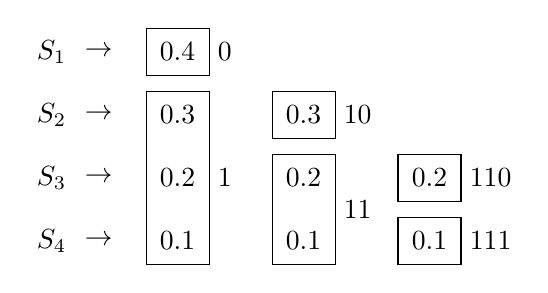
\begin{tikzpicture}[x=1cm, y=1cm]

		% Vertical and horizontal spacing parameters
		\def\xS{0}
		\def\xA{0.6}
		\def\xB{1.6}
		\def\xC{3.2}
		\def\xD{4.8}

		\def\yone{0}
		\def\ytwo{-0.8}
		\def\ythree{-1.6}
		\def\yfour{-2.4}

		% Box half-width and half-height
		\def\boxw{0.4}
		\def\boxh{0.3}

		% --- Symbols and Arrows ---
		\node at (\xS, \yone) {$S_1$};   \node at (\xA, \yone) {$\rightarrow$};
		\node at (\xS, \ytwo) {$S_2$};   \node at (\xA, \ytwo) {$\rightarrow$};
		\node at (\xS, \ythree) {$S_3$}; \node at (\xA, \ythree) {$\rightarrow$};
		\node at (\xS, \yfour) {$S_4$};  \node at (\xA, \yfour) {$\rightarrow$};

		% --- Column 1 ---
		\node (n11) at (\xB, \yone) {$0.4$};
		\draw ([xshift=-\boxw cm, yshift=\boxh cm]n11.center) rectangle ([xshift=\boxw cm, yshift=-\boxh cm]n11.center);
		\node[right, inner sep=3pt] at ([xshift=\boxw cm]n11.center) {$0$};

		\node (n21) at (\xB, \ytwo) {$0.3$};
		\node (n31) at (\xB, \ythree) {$0.2$};
		\node (n41) at (\xB, \yfour) {$0.1$};
		% Group box for S2, S3, S4
		\draw ([xshift=-\boxw cm, yshift=\boxh cm]n21.center) rectangle ([xshift=\boxw cm, yshift=-\boxh cm]n41.center);
		\node[right, inner sep=3pt] at ([xshift=\boxw cm]n31.center) {$1$};

		% --- Column 2 ---
		\node (n22) at (\xC, \ytwo) {$0.3$};
		\draw ([xshift=-\boxw cm, yshift=\boxh cm]n22.center) rectangle ([xshift=\boxw cm, yshift=-\boxh cm]n22.center);
		\node[right, inner sep=3pt] at ([xshift=\boxw cm]n22.center) {$10$};

		\node (n32) at (\xC, \ythree) {$0.2$};
		\node (n42) at (\xC, \yfour) {$0.1$};
		% Group box for S3, S4
		\draw ([xshift=-\boxw cm, yshift=\boxh cm]n32.center) rectangle ([xshift=\boxw cm, yshift=-\boxh cm]n42.center);
		\node[right, inner sep=3pt] at ([xshift=\boxw cm, yshift=-0.4cm]n32.center) {$11$};

		% --- Column 3 ---
		\node (n33) at (\xD, \ythree) {$0.2$};
		\draw ([xshift=-\boxw cm, yshift=\boxh cm]n33.center) rectangle ([xshift=\boxw cm, yshift=-\boxh cm]n33.center);
		\node[right, inner sep=3pt] at ([xshift=\boxw cm]n33.center) {$110$};

		\node (n43) at (\xD, \yfour) {$0.1$};
		\draw ([xshift=-\boxw cm, yshift=\boxh cm]n43.center) rectangle ([xshift=\boxw cm, yshift=-\boxh cm]n43.center);
		\node[right, inner sep=3pt] at ([xshift=\boxw cm]n43.center) {$111$};

	\end{tikzpicture}
\end{minipage}
\begin{minipage}{.4\linewidth}
	\renewcommand{\arraystretch}{1.2}
	\begin{tabular}{l l c}
		\rowcolor{black!10}
		\textbf{Symbol}       & \textbf{Code} & \textbf{Length ($l_i$)} \\
		$S_1 \rightarrow 0.4$ & 0             & 1                       \\
		$S_2 \rightarrow 0.3$ & 10            & 2                       \\
		$S_3 \rightarrow 0.2$ & 110           & 3                       \\
		$S_4 \rightarrow 0.1$ & 111           & 3                       \\
	\end{tabular}
\end{minipage}

\vspace*{20pt}

\begin{flalign*}
	\text{Average word length, }L &= \sum_i P_i l_i && \\
	&= 0.4 \times 1 + 0.3 \times 2 + 0.2 \times 3 + 0.1 \times 3 && \\
	&= 0.4 + 0.6 + 0.6 + 0.3 && \\
	&= 1.9 \text{ bits/symbol} &&
\end{flalign*}
\begin{flalign*}
	\text{Entropy, }H &= -\sum_i P_i \log_2 P_i && \\
	&= -(0.4 \log_2 0.4 + 0.3 \log_2 0.3 + 0.2 \log_2 0.2 + 0.1 \log_2 0.1) && \\
	&= 1.846 \text{ bits/symbol} && \\
	\text{Efficiency }\eta &= \dfrac{H}{L} = \dfrac{1.846}{1.9} && \\
	&= 0.9718 \Rightarrow 97.18\% && \\
	\text{Redundancy }&= 1 - \eta = 2.82\%
\end{flalign*}


\vspace{0.5cm}
\noindent \textbf{24.} A source emits 9 symbols with probabilities 0.49, 0.14, 0.14, 0.07, 0.07, 0.04, 0.02, 0.02, 0.01. Obtain the Shannon-Fano code. Find the average word length, entropy, efficiency and redundancy.

\textbf{Ans:}

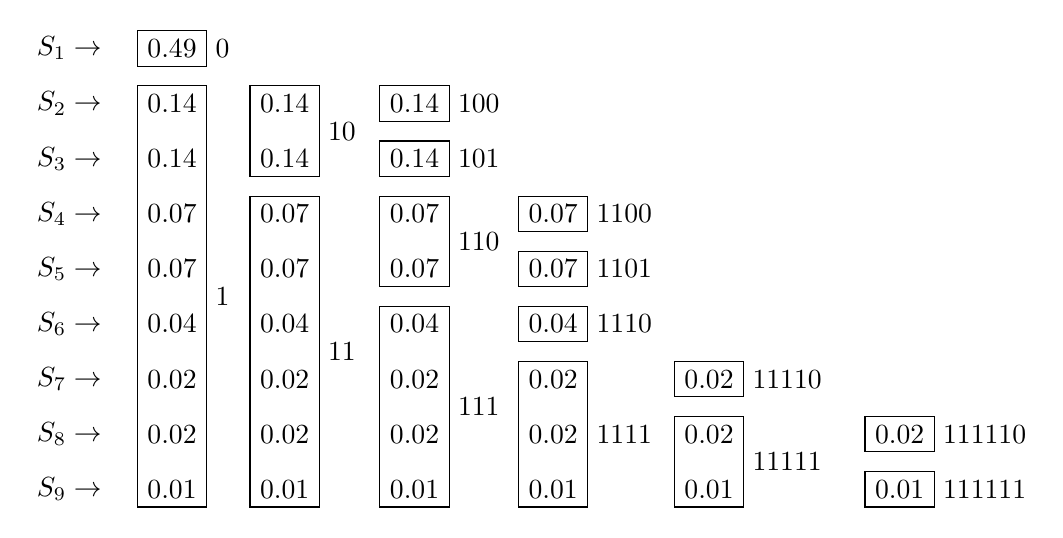
\begin{tikzpicture}[x=1.1cm, y=.7cm, >=stealth]

% Box dimensions (half-width and half-height)
\def\boxw{0.4}
\def\boxh{0.32}

% Macro to draw a grouping box and append the binary code label
% Usage: \gbox{x-coordinate}{start_y}{end_y}{label}
\newcommand{\gbox}[4]{
    \draw (#1-\boxw, #2+\boxh) rectangle (#1+\boxw, #3-\boxh);
    \node[right, inner sep=3pt] at (#1+\boxw, {(#2+#3)/2}) {#4};
}

% --- Column 0: Symbols ---
\foreach \y/\sym in {0/S_1, -1/S_2, -2/S_3, -3/S_4, -4/S_5, -5/S_6, -6/S_7, -7/S_8, -8/S_9} {
    \node[anchor=east] at (0.3, \y) {$\sym \rightarrow$};
}

% --- Column 1 ---
\def\xI{1.0}
\foreach \y/\val in {0/0.49, -1/0.14, -2/0.14, -3/0.07, -4/0.07, -5/0.04, -6/0.02, -7/0.02, -8/0.01} {
    \node at (\xI, \y) {\val};
}
\gbox{\xI}{0}{0}{0}
\gbox{\xI}{-1}{-8}{1}

% --- Column 2 ---
\def\xII{2.3}
\foreach \y/\val in {-1/0.14, -2/0.14, -3/0.07, -4/0.07, -5/0.04, -6/0.02, -7/0.02, -8/0.01} {
    \node at (\xII, \y) {\val};
}
\gbox{\xII}{-1}{-2}{10}
\gbox{\xII}{-3}{-8}{11}

% --- Column 3 ---
\def\xIII{3.8}
\foreach \y/\val in {-1/0.14, -2/0.14, -3/0.07, -4/0.07, -5/0.04, -6/0.02, -7/0.02, -8/0.01} {
    \node at (\xIII, \y) {\val};
}
\gbox{\xIII}{-1}{-1}{100}
\gbox{\xIII}{-2}{-2}{101}
\gbox{\xIII}{-3}{-4}{110}
\gbox{\xIII}{-5}{-8}{111}

% --- Column 4 ---
\def\xIV{5.4}
\foreach \y/\val in {-3/0.07, -4/0.07, -5/0.04, -6/0.02, -7/0.02, -8/0.01} {
    \node at (\xIV, \y) {\val};
}
\gbox{\xIV}{-3}{-3}{1100}
\gbox{\xIV}{-4}{-4}{1101}
\gbox{\xIV}{-5}{-5}{1110}
\gbox{\xIV}{-6}{-8}{1111}

% --- Column 5 ---
\def\xV{7.2}
\foreach \y/\val in {-6/0.02, -7/0.02, -8/0.01} {
    \node at (\xV, \y) {\val};
}
\gbox{\xV}{-6}{-6}{11110}
\gbox{\xV}{-7}{-8}{11111}

% --- Column 6 ---
\def\xVI{9.4}
\foreach \y/\val in {-7/0.02, -8/0.01} {
    \node at (\xVI, \y) {\val};
}
\gbox{\xVI}{-7}{-7}{111110}
\gbox{\xVI}{-8}{-8}{111111}

\end{tikzpicture}

\begin{table}[ht]
	\centering
	\renewcommand{\arraystretch}{1.2}
	\begin{tabular}{l l c}
		\rowcolor{black!10}
		\textbf{Symbol}        & \textbf{Code} & \textbf{Length ($l_i$)} \\
		$S_1 \rightarrow 0.49$ & 0             & 1                       \\
		$S_2 \rightarrow 0.14$ & 100           & 3                       \\
		$S_3 \rightarrow 0.14$ & 101           & 3                       \\
		$S_4 \rightarrow 0.07$ & 1100          & 4                       \\
		$S_5 \rightarrow 0.07$ & 1101          & 4                       \\
		$S_6 \rightarrow 0.04$ & 1110          & 4                       \\
		$S_7 \rightarrow 0.02$ & 11110         & 5                       \\
		$S_8 \rightarrow 0.02$ & 111110        & 6                       \\
		$S_9 \rightarrow 0.01$ & 111111        & 6                       \\
	\end{tabular}
\end{table}

Average word length, $L = \sum_i P_i l_i$
\begin{align*}
	 & = 0.49 \times 1 + 2 \times 0.14 \times 3 + 2 \times 0.07 \times 4 + 0.04 \times 4 + 0.02 \times 5 + 0.02 \times 6 + 0.01 \times 6 \\
	 & = 0.49 + 0.84 + 0.56 + 0.16 + 0.1 + 0.12 + 0.06 = 2.33 \text{ bits/symbol}
\end{align*}

Entropy, $H = -\sum_i P_i \log_2 P_i$
\begin{align*}
	 & = -\left( 0.49 \log_2 0.49 + 2 \times 0.14 \log_2 0.14 + 2 \times 0.07 \log_2 0.07 \right. \\
	 & \quad \left. + 0.04 \log_2 0.04 + 2 \times 0.02 \log_2 0.02 + 0.01 \log_2 0.01 \right)     \\
	 & = 2.314 \text{ bits/symbol}
\end{align*}

Efficiency $\eta = \dfrac{H}{L} = \dfrac{2.314}{2.33} = 0.9927 \Rightarrow 99.27\%$ \\

Redundancy $= 1 - \eta = 0.73\%$


\subsection{Huffman Coding (Minimum Redundancy Coding)}
\subsubsection*{Procedure}
\begin{enumerate}
	\item Arrange the source symbols in the decreasing order of probability.
	\item Check if number of source symbols $q = r + \alpha(r-1)$ is satisfied \& find the integer $\alpha$ (finite value). Otherwise add a dummy symbol with zero probability of occurrence to satisfy the condition. This step is not required if we use the binary coding method ($r=2$). In binary coding we always get $\alpha$ as an integer.
	\item Combine the last '$r$' symbols into a single composite signal whose probability of occurrence is equal to sum of probabilities of occurrence of the r-symbols involved in the step.
	\item Repeat steps 1 \& 3 on the resulting set of symbols until in the final step exactly r symbols are left.
	\item Assign codes freely to the last r-composite symbols and work backward to the source to arrive at the optimum code.
	\item Discard the codes of the dummy symbols.
\end{enumerate}

\subsubsection*{Problems}

\textbf{25.} Apply Huffman coding to the messages $S_0, S_1, S_2, S_3$ \& $S_4$ with probabilities 0.4, 0.2, 0.2, 0.1 \& 0.1.? Find the average word length, entropy, efficiency and redundancy.

\vspace*{10pt}
\textbf{Ans:}
\vspace*{10pt}
\begin{center}
	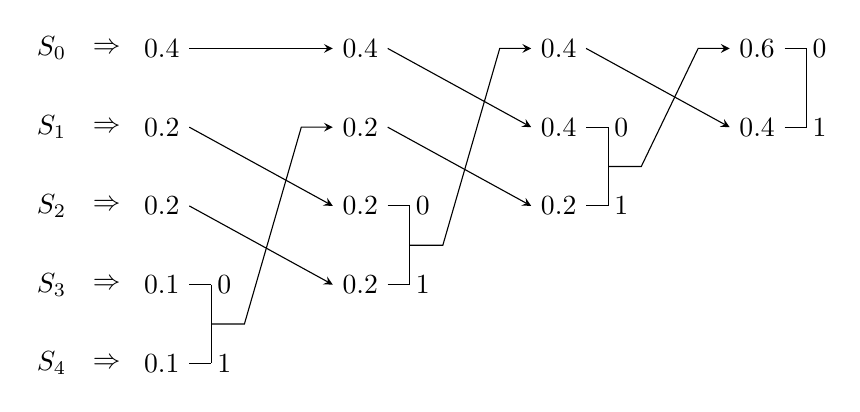
\begin{tikzpicture}[x=1.4cm, y=1cm, >=stealth]

		% Column 0: Symbols
		\node (S0) at (0, 0) {$S_0$};
		\node (S1) at (0, -1) {$S_1$};
		\node (S2) at (0, -2) {$S_2$};
		\node (S3) at (0, -3) {$S_3$};
		\node (S4) at (0, -4) {$S_4$};

		% Column 1: Arrows
		\foreach \y in {0,-1,-2,-3,-4} {
				\node at (0.5, \y) {$\Rightarrow$};
			}

		% Column 2: Initial Probabilities
		\node (P00) at (1.0, 0) {$0.4$};
		\node (P01) at (1.0, -1) {$0.2$};
		\node (P02) at (1.0, -2) {$0.2$};
		\node (P03) at (1.0, -3) {$0.1$};
		\node (P04) at (1.0, -4) {$0.1$};

		% Column 3: Stage 1
		\node (P10) at (2.8, 0) {$0.4$};
		\node (P11) at (2.8, -1) {$0.2$};
		\node (P12) at (2.8, -2) {$0.2$};
		\node (P13) at (2.8, -3) {$0.2$};

		% Column 4: Stage 2
		\node (P20) at (4.6, 0) {$0.4$};
		\node (P21) at (4.6, -1) {$0.4$};
		\node (P22) at (4.6, -2) {$0.2$};

		% Column 5: Stage 3
		\node (P30) at (6.4, 0) {$0.6$};
		\node (P31) at (6.4, -1) {$0.4$};


		% --- Brackets and Connections ---

		% Stage 1 (Col 2 to Col 3)
		\draw[->] (P00.east) -- (P10.west);
		\draw[->] (P01.east) -- (P12.west);
		\draw[->] (P02.east) -- (P13.west);

		\draw (P03.east) -- ++(0.2, 0) coordinate (B1T);
		\draw (P04.east) -- ++(0.2, 0) coordinate (B1B);
		\draw (B1T) -- (B1B) coordinate[midway] (B1M);
		\node[right, inner sep=2pt] at (B1T) {$0$};
		\node[right, inner sep=2pt] at (B1B) {$1$};
		\draw[->] (B1M) -- ++(.3, 0) -- ([xshift=-.4cm] P11.west) -- (P11.west);

		% Stage 2 (Col 3 to Col 4)
		\draw[->] (P10.east) -- (P21.west);
		\draw[->] (P11.east) -- (P22.west);

		\draw (P12.east) -- ++(0.2, 0) coordinate (B2T);
		\draw (P13.east) -- ++(0.2, 0) coordinate (B2B);
		\draw (B2T) -- (B2B) coordinate[midway] (B2M);
		\node[right, inner sep=2pt] at (B2T) {$0$};
		\node[right, inner sep=2pt] at (B2B) {$1$};
		\draw[->] (B2M) -- ++(.3, 0) -- ([xshift=-.4cm] P20.west) -- (P20.west);

		% Stage 3 (Col 4 to Col 5)
		\draw[->] (P20.east) -- (P31.west);

		\draw (P21.east) -- ++(0.2, 0) coordinate (B3T);
		\draw (P22.east) -- ++(0.2, 0) coordinate (B3B);
		\draw (B3T) -- (B3B) coordinate[midway] (B3M);
		\node[right, inner sep=2pt] at (B3T) {$0$};
		\node[right, inner sep=2pt] at (B3B) {$1$};
		\draw[->] (B3M) -- ++(.3, 0) -- ([xshift=-.4cm] P30.west) -- (P30.west);

		% Final Bracket (Col 5)
		\draw (P30.east) -- ++(0.2, 0) coordinate (B4T);
		\draw (P31.east) -- ++(0.2, 0) coordinate (B4B);
		\draw (B4T) -- (B4B);
		\node[right, inner sep=2pt] at (B4T) {$0$};
		\node[right, inner sep=2pt] at (B4B) {$1$};

	\end{tikzpicture}
\end{center}

\begin{table}[ht]
	\centering
	\renewcommand{\arraystretch}{1.2}
	\begin{tabular}{l l c}
		\rowcolor{black!10}
		\textbf{Symbol}       & \textbf{Code} & \textbf{Length ($l_i$)} \\
		$S_0 \rightarrow 0.4$ & 00            & 2                       \\
		$S_1 \rightarrow 0.2$ & 10            & 2                       \\
		$S_2 \rightarrow 0.2$ & 11            & 2                       \\
		$S_3 \rightarrow 0.1$ & 010           & 3                       \\
		$S_4 \rightarrow 0.1$ & 011           & 3                       \\
	\end{tabular}
\end{table}

Average word length, $L = \sum_i P_i l_i$
$$= 0.4 \times 2 + 2 \times 0.2 \times 2 + 2 \times 0.1 \times 3 = 0.8 + 0.8 + 0.6 = 2.2 \text{ bits/symbol}$$

Entropy, $H = -\sum_i P_i \log_2 P_i$
$$= -(0.4 \log_2 0.4 + 2 \times 0.2 \log_2 0.2 + 2 \times 0.1 \log_2 0.1) = 2.122 \text{ bits/symbol}$$

Efficiency $\eta = \dfrac{H}{L} = \dfrac{2.122}{2.2} = 0.9645 \Rightarrow 96.45\%$ \\

Redundancy $= 1 - \eta = 3.55\%$


\vspace{0.5cm}
\noindent \textbf{26.} Apply Huffman coding to the messages $S_0, S_1, S_2, S_3$ \& $S_4$ with probabilities 0.4, 0.2, 0.2, 0.1 \& 0.1? Find average word length, entropy, efficiency and redundancy. Choose $r=4$.

\textbf{Ans:}
$$q = r + \alpha(r-1)$$
$$\Rightarrow \alpha = \frac{q-r}{r-1} = \frac{5-4}{4-1} = \frac{1}{3}$$
Since $\alpha$ is not an integer, add one dummy variable, $S_5$ with probability 0. So now $q=6$.
$$\Rightarrow \alpha = \frac{q-r}{r-1} = \frac{6-4}{4-1} = \frac{2}{3}$$
Since $\alpha$ is not an integer, add one dummy variable, $S_6$ with probability 0. So now $q=7$.
$$\Rightarrow \alpha = \frac{q-r}{r-1} = \frac{7-4}{4-1} = \frac{3}{3} = 1$$

\begin{minipage}{.5\linewidth}
	\centering
	\vspace*{20pt}
	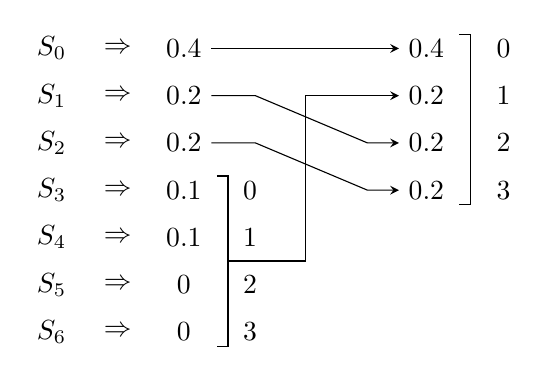
\begin{tikzpicture}[x=1.4cm, y=0.6cm, >=stealth]

		% Column 1: Symbols
		\node (S0) at (0, 0) {$S_0$};
		\node (S1) at (0, -1) {$S_1$};
		\node (S2) at (0, -2) {$S_2$};
		\node (S3) at (0, -3) {$S_3$};
		\node (S4) at (0, -4) {$S_4$};
		\node (S5) at (0, -5) {$S_5$};
		\node (S6) at (0, -6) {$S_6$};

		% Column 2: Arrows
		\foreach \y in {0,-1,-2,-3,-4,-5,-6} {
				\node at (0.6, \y) {$\Rightarrow$};
			}

		% Column 3: Initial Probabilities
		\node (P0) at (1.2, 0) {$0.4$};
		\node (P1) at (1.2, -1) {$0.2$};
		\node (P2) at (1.2, -2) {$0.2$};
		\node (P3) at (1.2, -3) {$0.1$};
		\node (P4) at (1.2, -4) {$0.1$};
		\node (P5) at (1.2, -5) {$0$};
		\node (P6) at (1.2, -6) {$0$};

		% Inner Bracket (grouping the bottom 4 probabilities)
		\draw (1.5, -2.7) -- (1.6, -2.7) -- (1.6, -6.3) -- (1.5, -6.3);

		% Inner Codes (assigned to the grouped probabilities)
		\node (C3) at (1.8, -3) {$0$};
		\node (C4) at (1.8, -4) {$1$};
		\node (C5) at (1.8, -5) {$2$};
		\node (C6) at (1.8, -6) {$3$};

		% Column 4: Reduced Probabilities
		\node (N0) at (3.4, 0) {$0.4$};
		\node (N1) at (3.4, -1) {$0.2$};
		\node (N2) at (3.4, -2) {$0.2$};
		\node (N3) at (3.4, -3) {$0.2$};

		% Outer Bracket (grouping the reduced probabilities)
		\draw (3.7, 0.3) -- (3.8, 0.3) -- (3.8, -3.3) -- (3.7, -3.3);

		% Outer Codes
		\node (R0) at (4.1, 0) {$0$};
		\node (R1) at (4.1, -1) {$1$};
		\node (R2) at (4.1, -2) {$2$};
		\node (R3) at (4.1, -3) {$3$};

		% --- Connecting Lines ---

		% 0.4 to 0.4 (Straight horizontal line)
		\draw[->] (P0.east) -- (N0.west);

		% Bracket to 0.2 (Orthogonal routing: Right, Up, Right)
		% The middle of the inner bracket is at y = -4.5
		\draw[->] (1.6, -4.5) -- (2.3, -4.5) -- (2.3, -1) -- (N1.west);

		% 0.2 to 0.2 (Angled crossing line)
		\draw[->] (P1.east) -- ++(0.4, 0) -- ([xshift=-0.4cm]N2.west) -- (N2.west);

		% 0.2 to 0.2 (Angled crossing line)
		\draw[->] (P2.east) -- ++(0.4, 0) -- ([xshift=-0.4cm]N3.west) -- (N3.west);

	\end{tikzpicture}
\end{minipage}%
\hfill
\begin{minipage}{.5\linewidth}
	\centering
	\renewcommand{\arraystretch}{1.2}
	\begin{tabular}{l l c}
		\rowcolor{black!10}
		\textbf{Symbol}       & \textbf{Code} & \textbf{Length ($l_i$)} \\
		$S_0 \rightarrow 0.4$ & 0             & 1                       \\
		$S_1 \rightarrow 0.2$ & 1             & 1                       \\
		$S_2 \rightarrow 0.2$ & 2             & 1                       \\
		$S_3 \rightarrow 0.1$ & 30            & 2                       \\
		$S_4 \rightarrow 0.1$ & 31            & 2                       \\
	\end{tabular}
\end{minipage}

\vspace*{10pt}
\begin{flalign*}
	\text{Average word length, }L & = \sum_i P_i l_i                                                           &  & \\
	                              & = 0.4 \times 1 + 0.2 \times 1 + 0.2 \times 1 + 0.1 \times 2 + 0.1 \times 2 &  & \\
	                              & = 0.4 + 0.2 + 0.2 + 0.2 + 0.2                                              &  & \\
	                              & = 1.2 \text{ symbols/message}                                              &  &
\end{flalign*}
\begin{flalign*}
	\text{Entropy, }H       & = -\sum_i P_i \log_2 P_i                                                        &  & \\
	                        & = -(0.4 \log_2 0.4 + 2 \times 0.2 \log_2 0.2 + 2 \times 0.1 \log_2 0.1)         &  & \\
	                        & = 2.122 \text{ bits/message}                                                    &  & \\
	\text{Efficiency } \eta & = \dfrac{H}{L \log_2 r} = \dfrac{2.122}{1.2 \times \log_2 4}                    &  & \\
	                        & = \dfrac{2.122}{1.2 \times 2} = \dfrac{2.122}{2.4} = 0.8842 \Rightarrow 88.42\% &  & \\
	\text{Redundancy }      & = 1 - \eta = 11.58\%                                                            &  &
\end{flalign*}

\subsection{Lempel - Ziv Algorithm}
This source coding algorithm doesn't need source statistics (source probability). Lempel-Ziv coding is a variable to fixed length source coding algorithm proposed by Abraham Lempel \& Jacob Ziv in 1977. This algorithm is intrinsically adaptable \& simpler to implement than Huffman source coding algorithm.

\subsubsection*{Procedure}
\begin{enumerate}
	\item The comparison of an arbitrary binary sequence is possible by encoding a series of 1s \& 0s as some previous strings (prefix string).
	\item New string is formed by the process known as parsing. \\
	      Parsing = prefix string + new bits
	\item Thus parsing becomes a potential prefix string for future strings. The variable length blocks thus obtained are known as phrases.
	\item Then phrases are listed in a dictionary or code book, which stores the existing phrases \& their locations. In encoding a new phrase we specify the location of the existing phrase in the code book \& append the new letter.
\end{enumerate}

\subsubsection*{Advantages}
\begin{enumerate}
	\item This algorithm uses fixed length codes to represent a variable number of source symbols.
	\item This coding method is suitable for synchronous transmission.
	\item It is now used as the standard algorithm for file compression.
	\item Achieves a compression of 55\% [Huffman Coding 43\%].
\end{enumerate}

\subsection{Run Length Encoding}
It is used to reduce the size of a repeating string. This repeating string is called run. RLE encodes a run of symbols into two bytes (Count + Symbol). RLE cannot achieve high compression ratio compared to other compression methods. But it is easy to implement and quick to execute.

\textbf{Example:} \\
Consider the bit string 11111111111111100000000000000000001111. Encode this in run length encoding.

Original: \texttt{11111111111111100000000000000000001111} (38 bits) \\
(Count, Symbol) $= (15, 1), (19, 0), (4, 1)$ \\
Encoded: \texttt{(01111, 1), (10011, 0), (00100, 1)} (18 bits)

\end{document}
